\chapter {Ergebnisse}

\section{$\alpha_p$-Studie (PH)}

Im Rahmen der $\alpha_p$-Studie wurden zunächst 3 Proben bei verschiedenen Temperaturen unterhalb der $\beta$-Transus Temperatur (995$^\circ$C für Ti-6242) wärmebehandelt. Ziel war die Einstellung einer bimodalen Mikrostruktur, sowie die Bestimmung des $\alpha_p$-Volumenanteils. Es wurden 4 Temperaturen (990$^\circ$C, 983$^\circ$C, 975$^\circ$C und 960$^\circ$C) ausgewählt, bei denen die Proben für eine Stunde im Ofen wärmebehandelt und anschließend auf Raumtemperatur luftgekühlt wurden. Zusätzlich wurde eine Vergleichsprobe oberhalb der $\beta$-Transus-Temperatur bei 1015$^\circ$C für 30 Minuten geglüht und anschließend in Wasser abgeschreckt, um ein vollmartensitisches Gefüge einzustellen. Die Auswertung dieser Proben unter dem Lichtmikroskop sind in Abbildung \ref{fig:abbildung-8} aufgeführt. 

\begin{figure}
	\centering
	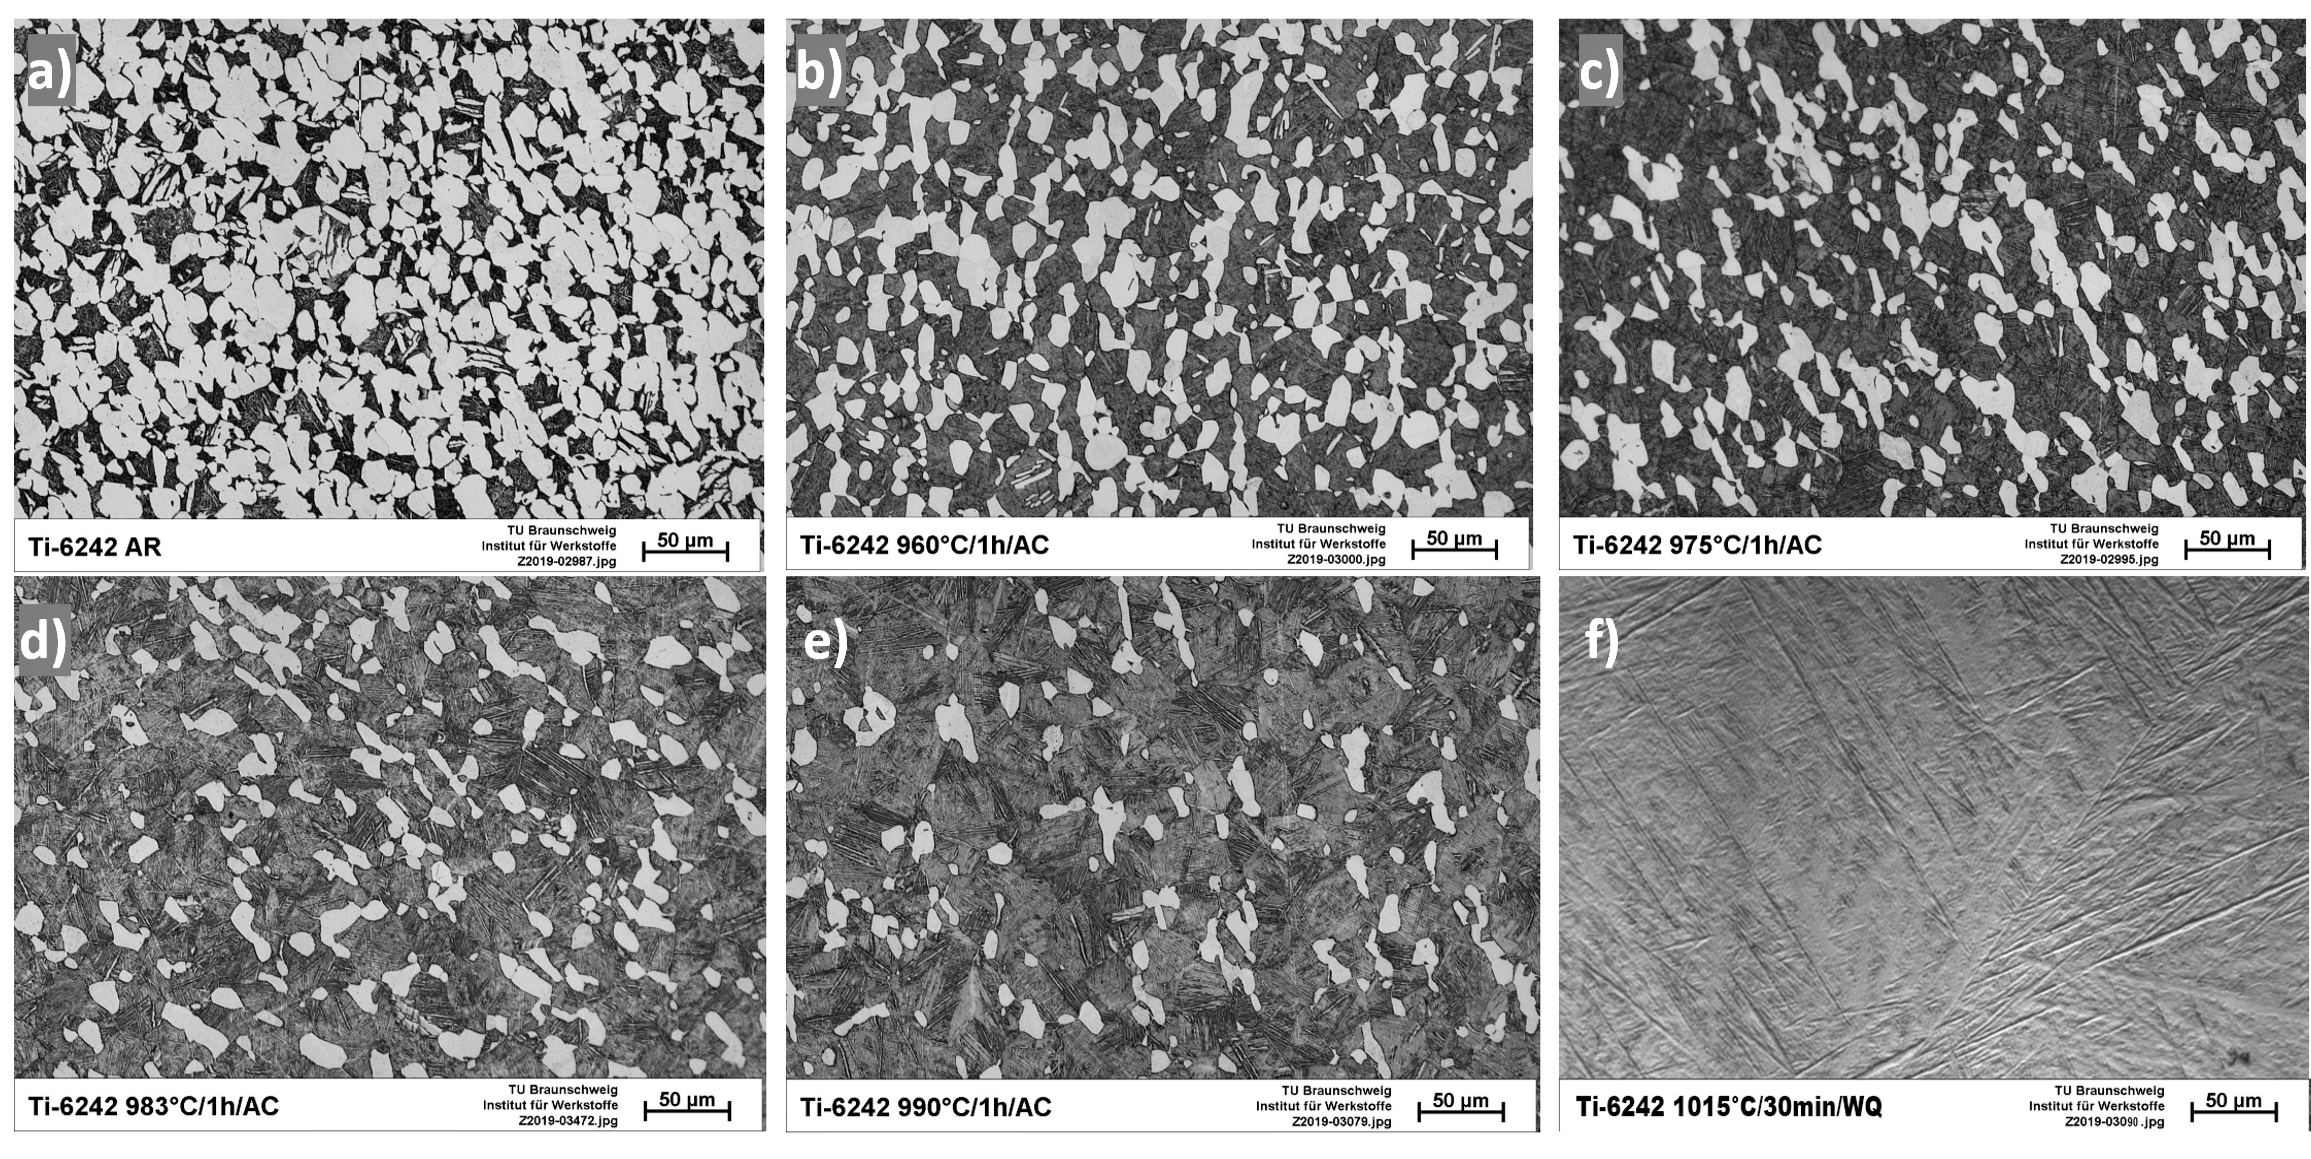
\includegraphics[width=1.0\linewidth]{./Bilder/Abbildung 8}
	\caption[Abbildung 8]{Mikrostrukturen der verwendeten Ti-6242 Legierung vor und nach der ersten Wärmebehandlung bei verschiedenen Temperaturen, a) Mikrostruktur vor Wärmebehandlung, b) 960$^\circ$C/1h/AC, c) 975$^\circ$C/1h/AC, d) 983$^\circ$C/1h/AC, e) 990$^\circ$C/1h/AC, f) 1015$^\circ$C/30min/WQ vollmartensitisches Gefüge}
	\label{fig:abbildung-8}
\end{figure}

Ein Überblick über die in der bimodalen Mikrostruktur auftretenden Gefügebestandteile zeigt die Abbildung \ref{fig:abbildung-20}.

\begin{figure}
	\centering
	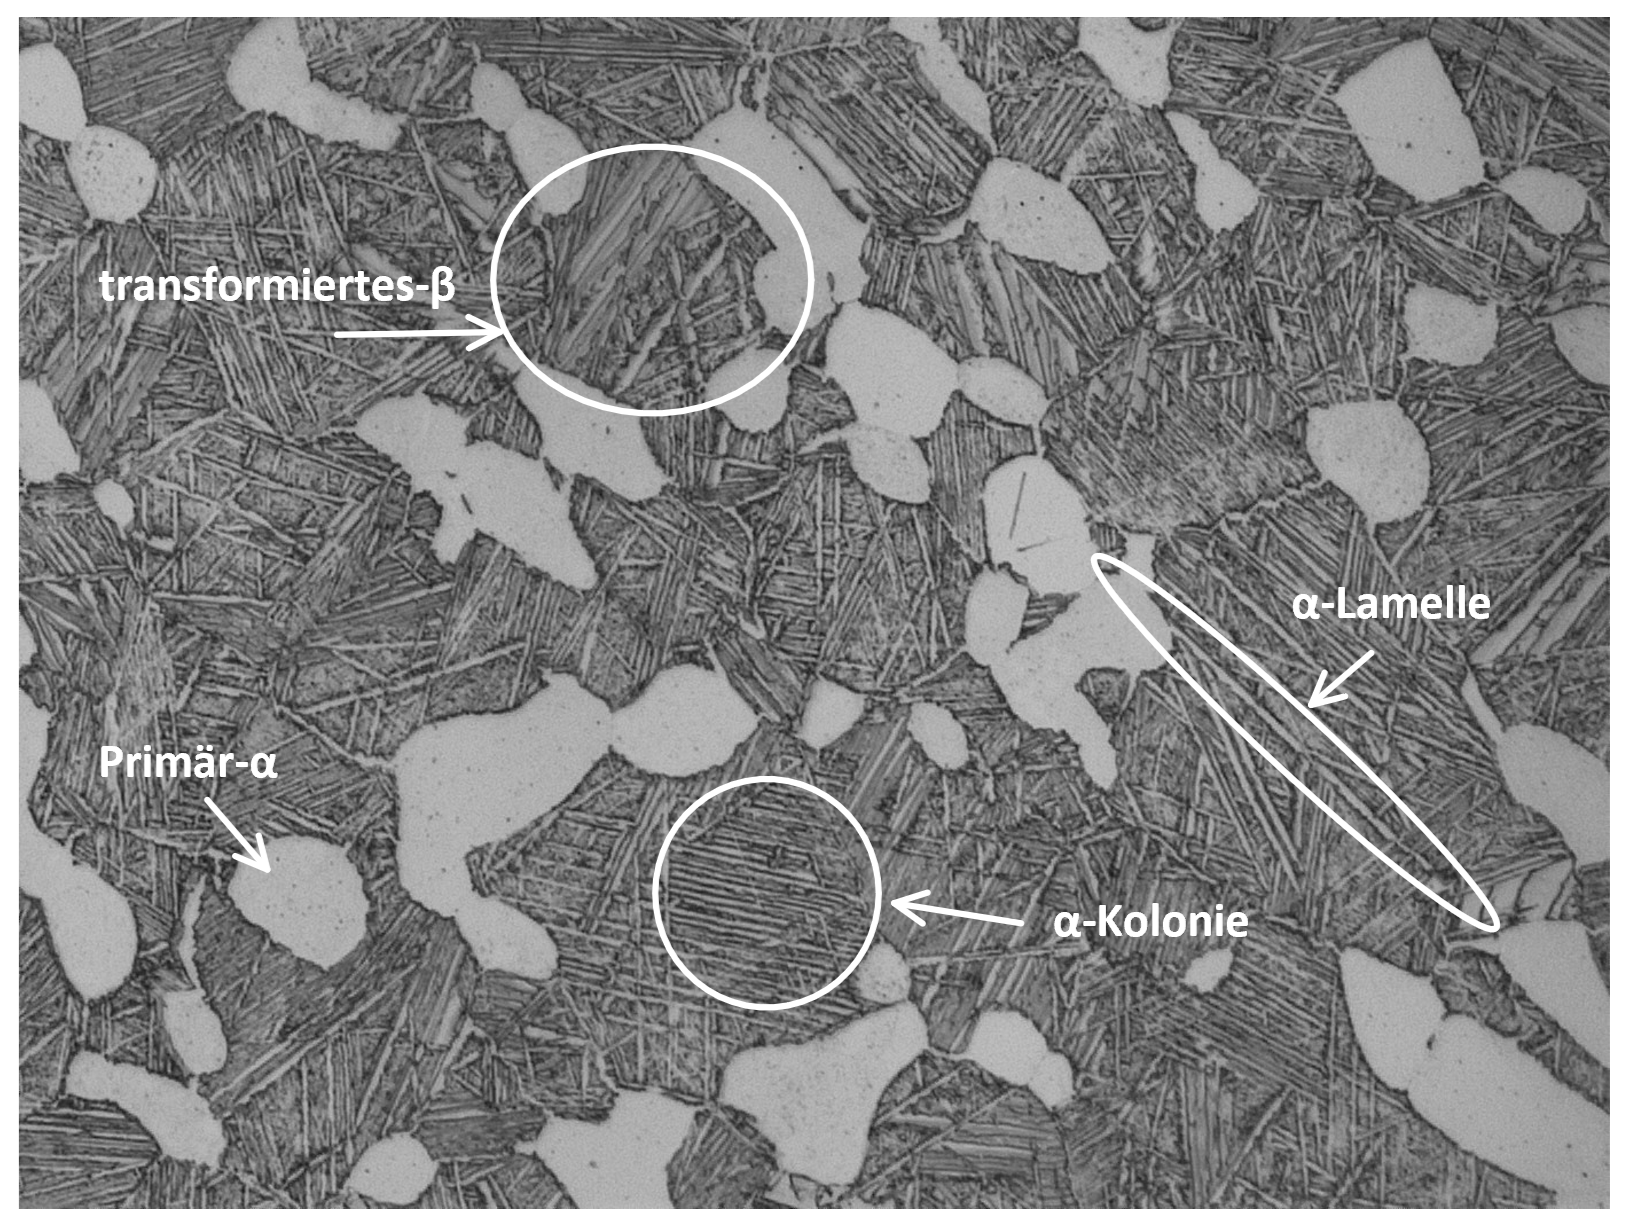
\includegraphics[width=0.9\linewidth]{./Bilder/Abbildung 20}
	\caption[Abbildung 20]{Gefügebestandteile in bimodaler Mikrostruktur}
	\label{fig:abbildung-20}
\end{figure}

Die Ergebnisse der Bestimmung des $\alpha_p$-Volumenanteils mittels Bildbearbeitungsprogramm sind in Tabelle \ref{Tabelle 4} aufgeführt. Laut Lütjering und Williams liegt der optimale $\alpha_p$-Volumenanteil zur Steigerung der Zugfestigkeitswerte zwischen 10 und 20 \% \cite{Lutjering.2007}.

\begin{table}
	\centering
	\begin{tabular}{|c|c|}
		\hline 
		Probe & Primär-$\alpha$ in \% \\ 
		\hline 
		AR & 62 \\ 
		\hline 
		960$^\circ$C/1h/AC & 37 \\ 
		\hline 
		975$^\circ$C/1h/AC & 26 \\ 
		\hline 
		983$^\circ$C/1h/AC & 16 \\ 
		\hline 
		990$^\circ$C/1h/AC & 9 \\ 
		\hline 
		1015$^\circ$C/30min/WQ & 0 \\ 
		\hline 
	\end{tabular} 
	\caption{$\alpha_p$-Volumenanteile der ersten Wärmebehandlungen mit einer Genauigkeit von 3\%}
	\label{Tabelle 4}
\end{table}

Die Auswertung hat ergeben, dass der angestrebte $\alpha_p$-Volumenanteil mit der Wärmebehandlung bei 983$^\circ$C für $1 h$ mit anschließender Luftkühlung erreicht wurde. Die vollmartensitische Probe hat wie erwartet keinen sichtbaren $\alpha_p$-Anteil aufgewiesen.

Des Weiteren wurde an der ersten Probenreihe eine Härteprüfung durchgeführt. Die Ergebnisse sind in Tabelle \ref{Tabelle 5} aufgeführt. 

\begin{table}
	\centering
	\begin{tabular}{|c|c|}
		\hline 
		Probe & Härte in HV \\ 
		\hline 
		AR & 331 \\ 
		\hline 
		960$^\circ$C/1h/AC & 345 \\ 
		\hline 
		975$^\circ$C/1h/AC & 344 \\ 
		\hline 
		983$^\circ$C/1h/AC & 344 \\ 
		\hline 
		990$^\circ$C/1h/AC & 350 \\ 
		\hline 
		1015$^\circ$C/30min/WQ & 403 \\ 
		\hline 
	\end{tabular} 
    \caption{Härtewerte der ersten Probenreihe in HV und ihre Standardabweichung}
    \label{Tabelle 5}
\end{table}

Nach der ersten Wärmebehandlung war bei den Proben mit bimodaler Mikrostruktur nur eine geringe Härtesteigerung gegenüber der AR-Probe festzustellen. 
Die Probe mit vollmartensitischem Gefüge hat dagegen eine beträchtliche Härtesteigerung gezeigt. Dies kann durch die feinere Struktur des Martensits und dadurch erhöhte Grenzflächendichte begründet werden. Sie wurde aber im Rahmen der gewählten Strategien nicht weiter verfolgt, da bimodale Gefüge im Hinblick auf die zu erreichende Bruchdehnung (mind. 10\%) eine bessere Basis darstellen.

\section{Short Time Duplex Heat Treatment (STDA - short Time Duplex Anneal) (PH)}

Im nächsten Schritt wurde versucht, die STDA Wärmebehandlung von der $\alpha$+$\beta$ Legierung Ti-6Al-4V auf die near-$\alpha$-Legierung Ti-6Al-2Sn-4Zr-2Mo zu übertragen. Ziel war es zunächst in einem zweiten Prozessschritt Martensit in der $\beta$-Phase zu erzeugen. Dafür wurden die Proben mit bimodalen Mikrostrukturen aus der ersten Wärmebehandlung erneut bei 930$^\circ$C im Ofen für 8 Minuten geglüht und anschließend wassergekühlt. Die Auswertung unter dem Lichtmikroskop ist in Abbildung \ref{fig:abbildung-9} zusammengefasst.

\begin{figure}
	\centering
	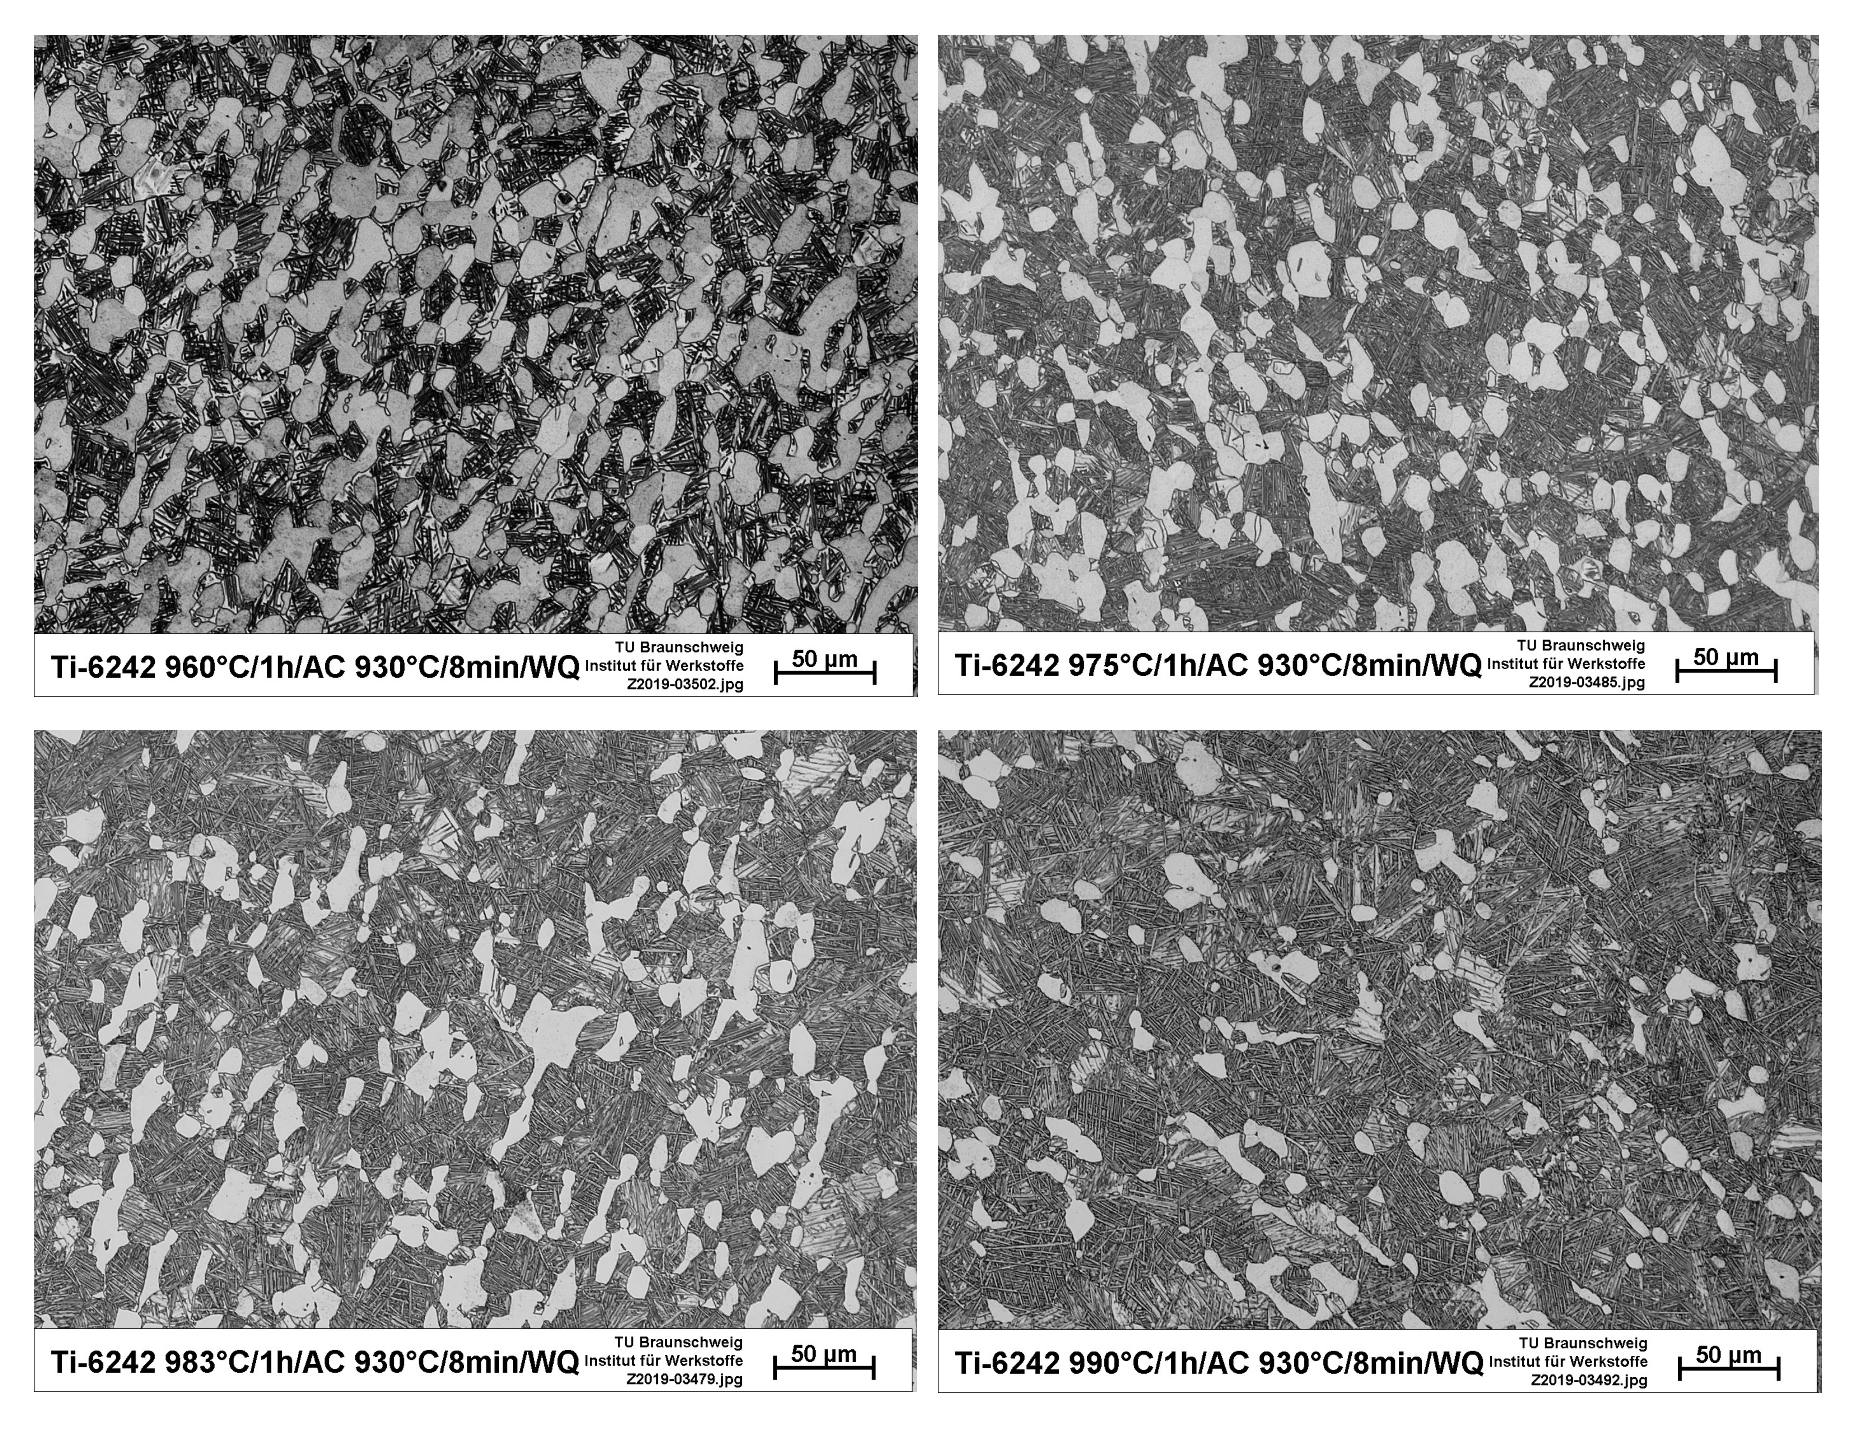
\includegraphics[width=0.9\linewidth]{./Bilder/Abbildung 9}
	\caption[Abbildung 9]{Mikrostrukturen von Ti-6242 nach dem zweiten Prozessschritt}
	\label{fig:abbildung-9}
\end{figure}

Nach dem zweiten Prozessschritt konnte keine Veränderung der Mikrostrukturen unter dem Lichtmikroskop zum ersten Schritt festgestellt werden. Daher wurden die Proben unter dem Rasterelektronenmikroskop (REM) näher untersucht, um festzustellen, ob sich Martensit in der $\beta$-Phase geformt hat. Die Ergebnisse sind in Abbildungen \ref{fig:abbildung-10} -- \ref{fig:abbildung-13} aufgeführt. 

Das Martensit in der $\beta$-Phase bildet sich nadelförmig aus. Diese Martensitnadeln entstehen häufig in einem orthogonalem Winkel zueinander. In Abbildung \ref{fig:abbildung-21} sind Beispiele für martensitische Strukturen innerhalb der $\beta$-Phase hervorgehoben.

\begin{figure}
	\centering
	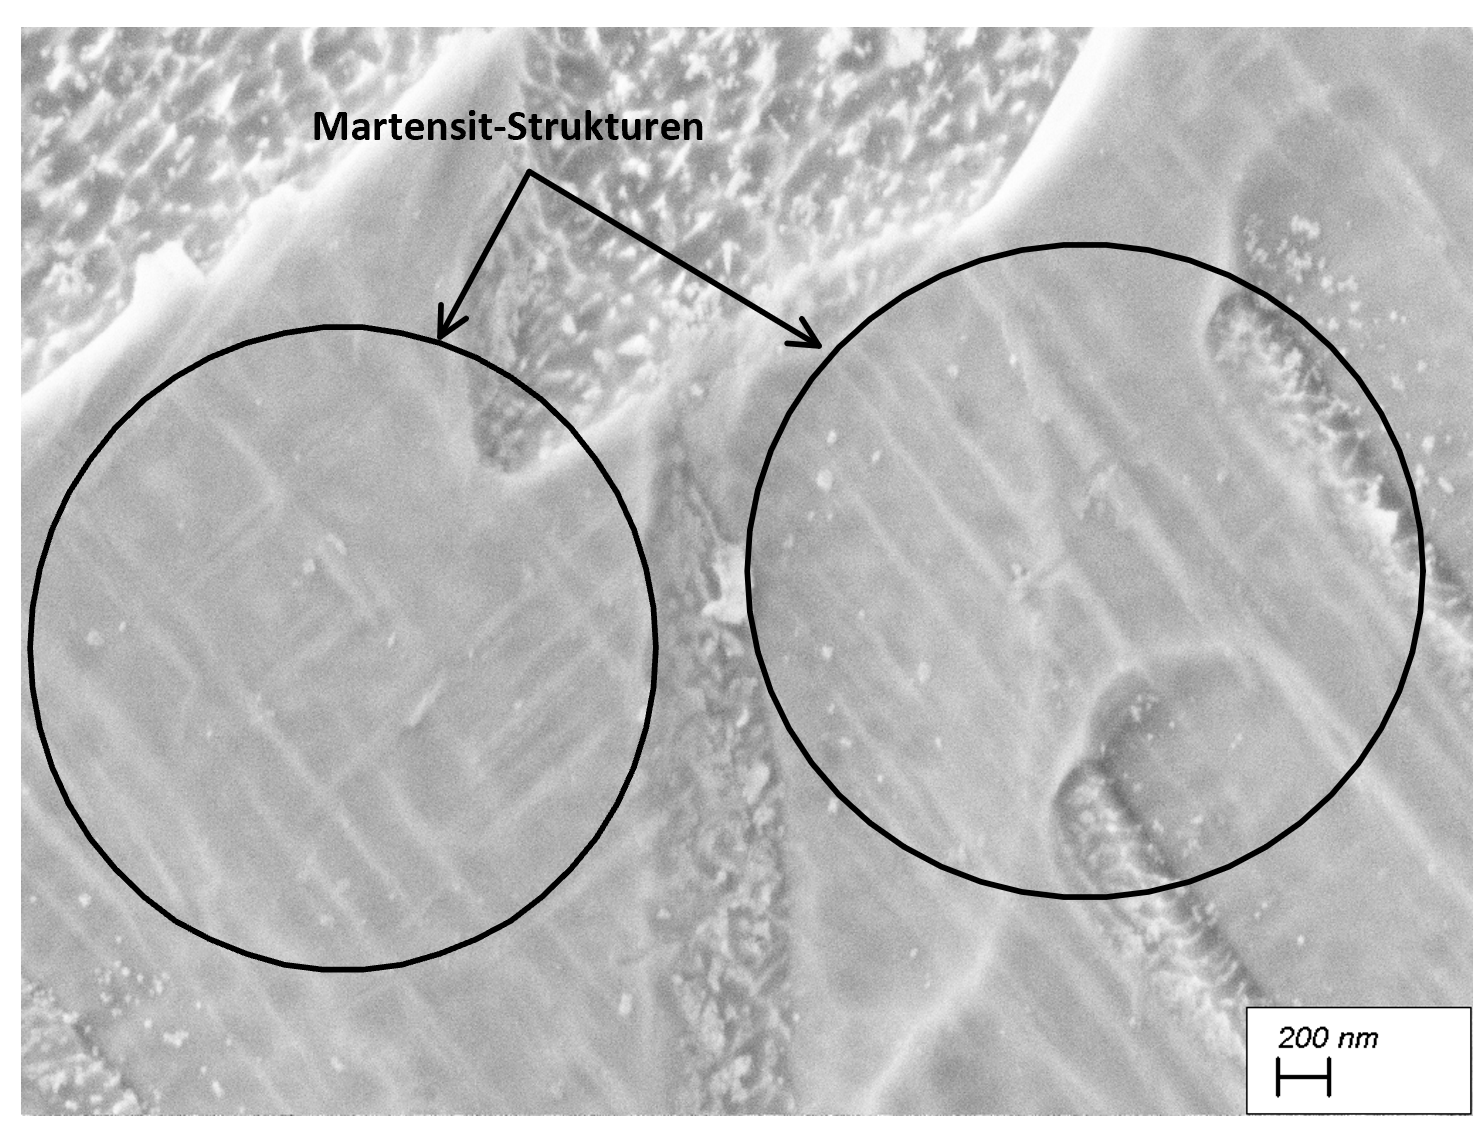
\includegraphics[width=0.8\linewidth]{./Bilder/Abbildung 21}
	\caption[Abbildung]{Martensit-Strukturen in der $\beta$-Phase}
	\label{fig:abbildung-21}
\end{figure}

\begin{figure}
	\centering
	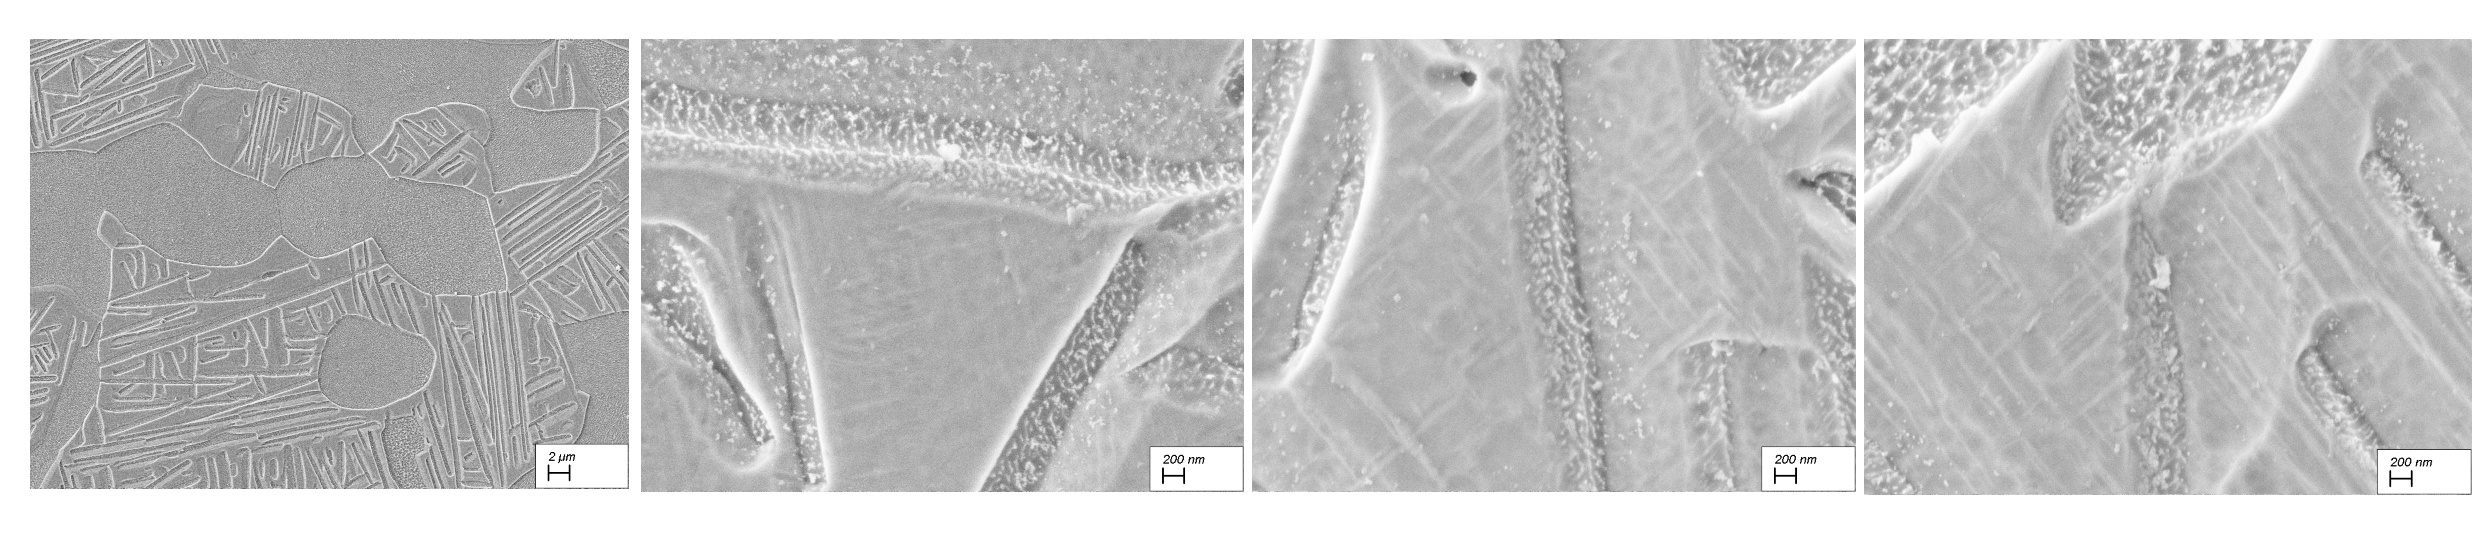
\includegraphics[width=1.0\linewidth]{./Bilder/Abbildung 10}
	\caption[Abbildung 10]{960$^\circ$C/1h/AC + 930$^\circ$C/8min/WQ, REM, Randbereich}
	\label{fig:abbildung-10}
\end{figure}

\begin{figure}
	\centering
	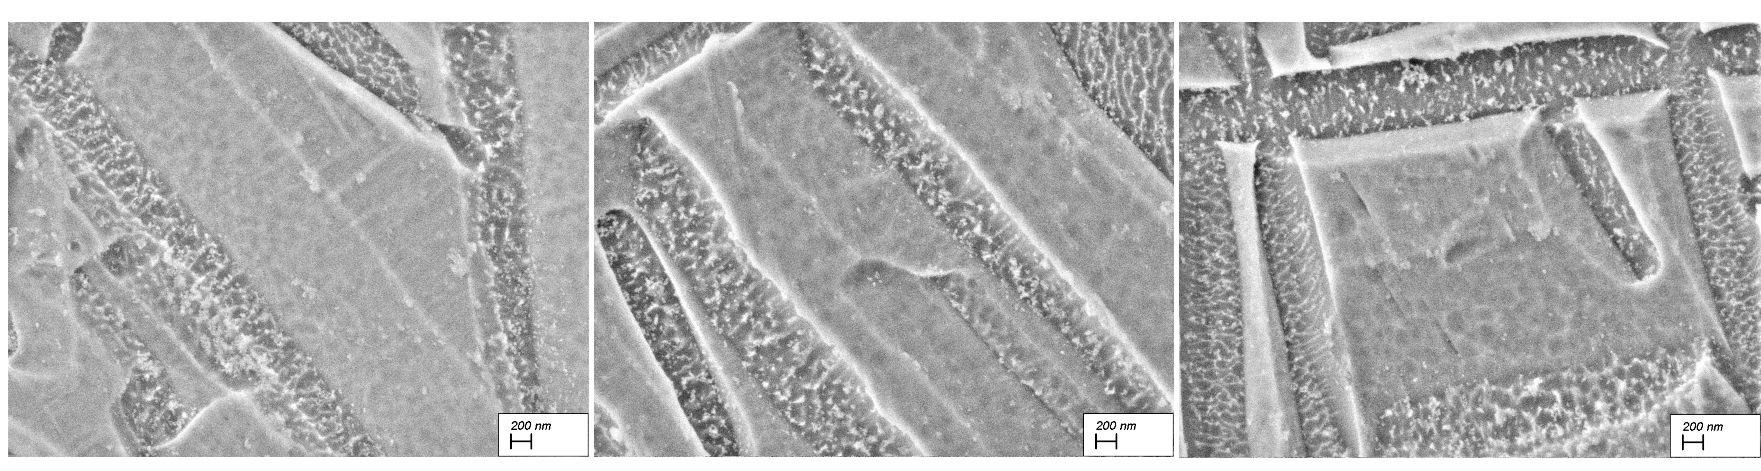
\includegraphics[width=1.0\linewidth]{./Bilder/Abbildung 11}
	\caption[Abbildung 11]{975$^\circ$C/1h/AC + 930$^\circ$C/8min/WQ, REM unter verschiedenen Vergrößerungen, Randbereich}
	\label{fig:abbildung-11}
\end{figure}

\begin{figure}
	\centering
	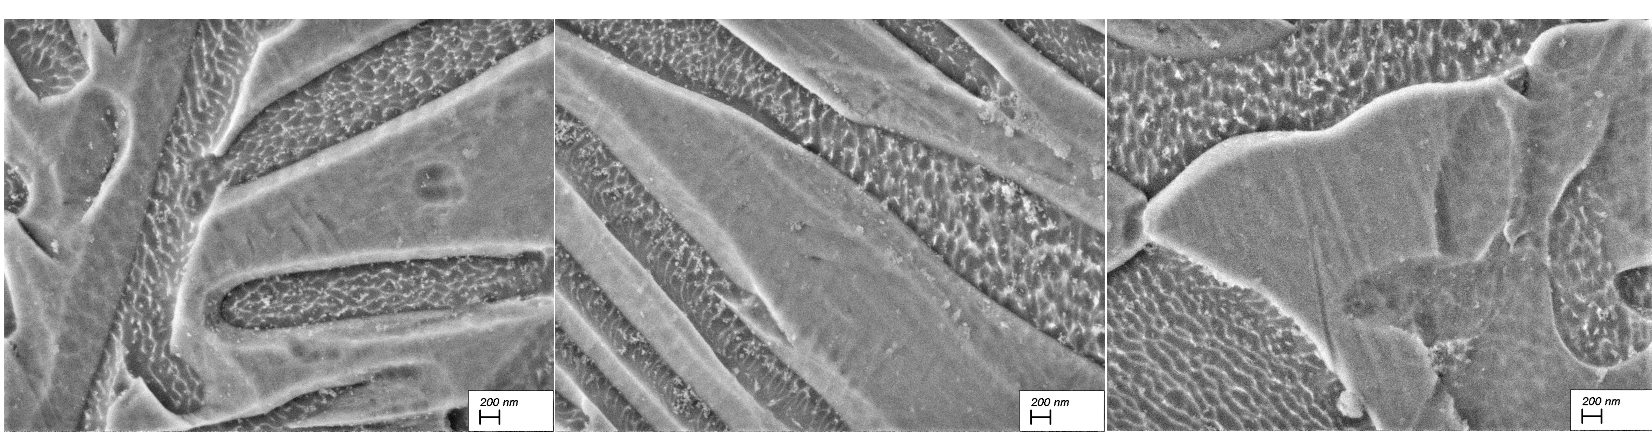
\includegraphics[width=1.0\linewidth]{./Bilder/Abbildung 12}
	\caption[Abbildung 12]{983$^\circ$C/1h/AC + 930$^\circ$C/8min/WQ, REM unter verschiedenen Vergrößerungen, Randbereich}
	\label{fig:abbildung-12}
\end{figure}

\begin{figure}
	\centering
	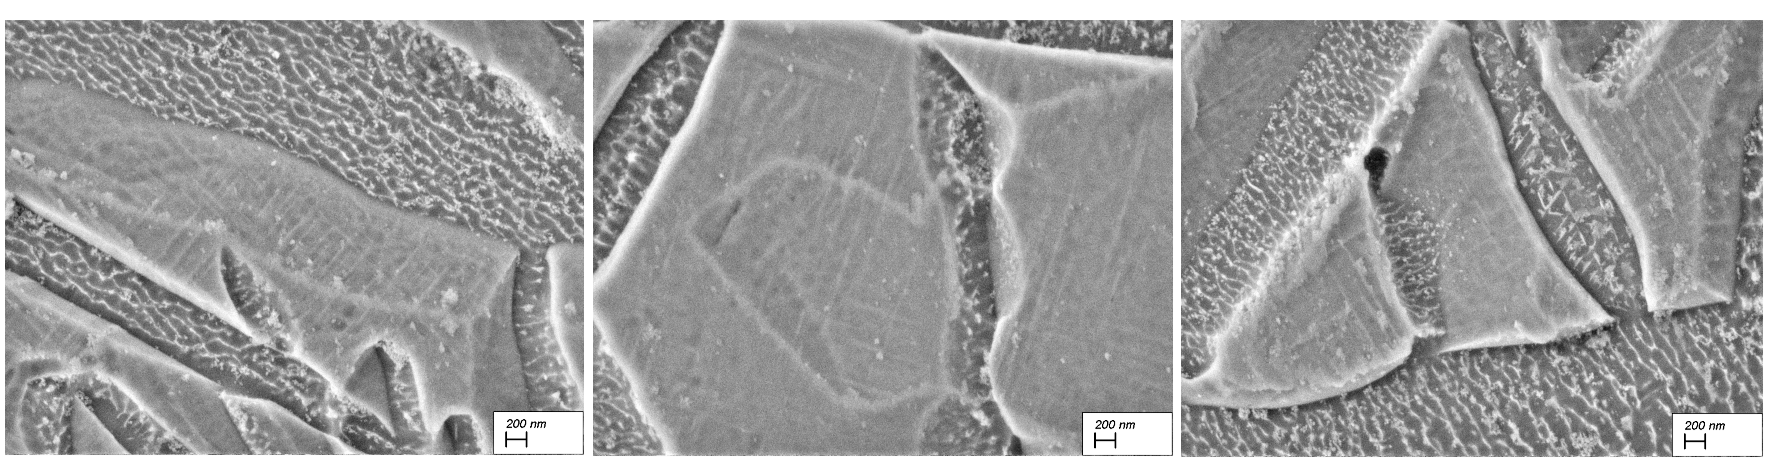
\includegraphics[width=1.0\linewidth]{./Bilder/Abbildung 13}
	\caption[Abbildung 13]{990$^\circ$C/1h/AC + 930$^\circ$C/8min/WQ, REM unter verschiedenen Vergrößerungen, Randbereich}
	\label{fig:abbildung-13}
\end{figure}

In den Abbildungen \ref{fig:abbildung-10} -- \ref{fig:abbildung-13} ist zu erkennen, dass lediglich die Proben der Temperaturenreihe mit 960$^\circ$C und 990$^\circ$C ansatzweise martensitische Strukturen im Randbereich aufweisen. In den Proben der Temperaturen 975$^\circ$C und 983$^\circ$C sind nur vereinzelt Martensitnadeln zu erkennen. Da diese Temperaturen zwischen 960$^\circ$C und 990$^\circ$C liegen, ist davon auszugehen, dass auch diese Proben stellenweise ausgeprägte Martensitstrukturen aufweisen, jedoch bei der Auswertung unter dem REM nicht gefunden wurden. Die Ergebnisse der folgenden Härteprüfung lässt ebenfalls auf diese Vermutung schließen. Die Qualität der Probenpräparation kann ebenfalls einen Einfluss auf die Sichtbarkeit der Strukturen haben.

Die Härteprüfung dieser Probenreihe ist in Tabelle \ref{Tabelle 6} zusammengefasst, zeigt jedoch bei keiner Probe eine sichtbare Härtesteigerung gegenüber den Werten nach der ersten Wärmebehandlung aus Tabelle \ref{Tabelle 5}.

\begin{table}
	\centering
	\begin{tabular}{|c|c|}
		\hline 
		Probe & Härte in HV \\ 
		\hline 
		960$^\circ$C/1h/AC + 930$^\circ$C/8min/WQ & 350 \\ 
		\hline 
		975$^\circ$C/1h/AC + 930$^\circ$C/8min/WQ & 345 \\ 
		\hline 
		983$^\circ$C/1h/AC + 930$^\circ$C/8min/WQ & 349 \\ 
		\hline 
		990$^\circ$C/1h/AC + 930$^\circ$C/8min/WQ & 352 \\ 
		\hline 
    \end{tabular} 
	\caption{Ergebnisse der Härteprüfung der zweiten Probenreihe}
	\label{Tabelle 6}
\end{table}

Die Ergebnisse dieser Probenreihe entsprach nicht den Erwartungen, da es nur stellenweise zur Martensitbildung im Randbereich kam. Daher wurde dieser zweite Schritt der Wärmebehandlung genauer verfolgt. Ab diesem Punkt wurde im ersten Schritt nur noch mit der Temperatur gearbeitet, die in der $\alpha_p$-Studie als Kandidat für den besten $\alpha_p$-Volumenanteil, in Hinblick auf die Zugwerte, ermittelt wurde (983$^\circ$C). 

Um den vorherigen Schritt genauer zu analysieren und optimieren zu können, wurden 3 neue Proben wärmebehandelt. Es wurde daher im zweiten Schritt die Haltezeit der vorherigen Probe verdoppelt. Zusätzlich wurden 2 Proben bei den zwei verschiedenen Haltezeiten (8 und 16 min) mit einer Temperatur geglüht, die um 20$^\circ$C auf 950$^\circ$C angehoben wurde. Dadurch sollten die Einflussfaktoren Temperatur und Haltezeit auf diesen Behandlungsschritt näher untersucht werden, um herauszufinden, warum es nur stellenweise zur Martensitbildung kam. Die Auswertung unter dem Lichtmikroskop ist in Abbildung \ref{fig:abbildung-14} zusammengefasst. 

\begin{figure}
\centering
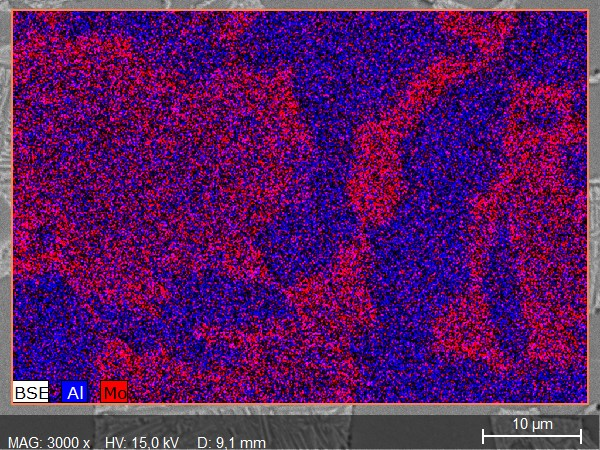
\includegraphics[width=0.9\linewidth]{./Bilder/Abbildung 14}
\caption[Abbildung 14]{Mikrostrukturen nach der Anpassung der Temperatur und Haltezeit im zweiten Wärmebehandlungsschritt}
\label{fig:abbildung-14}
\end{figure}

Die Proben, die im zweiten Schritt bei 930$^\circ$C geglüht wurden, weisen in ihrer Mikrostruktur keine offensichtlichen Unterschiede zur vorherigen Probenreihe (Abbildung \ref{fig:abbildung-9})auf. Die Proben, die im zweiten Schritt bei 950$^\circ$C geglüht wurden weisen eine Veränderung in der $\beta$-Phase auf. So scheint der $\beta$-Phasenanteil zwischen den $\alpha$-Lamellen gewachsen zu sein. Eine Gegenüberstellung der Proben bei 950$^\circ$C und 930$^\circ$C unter dem Lichtmikroskop ist in Abbildung \ref{fig:abbildung-15} zu sehen.

\begin{figure}
\centering
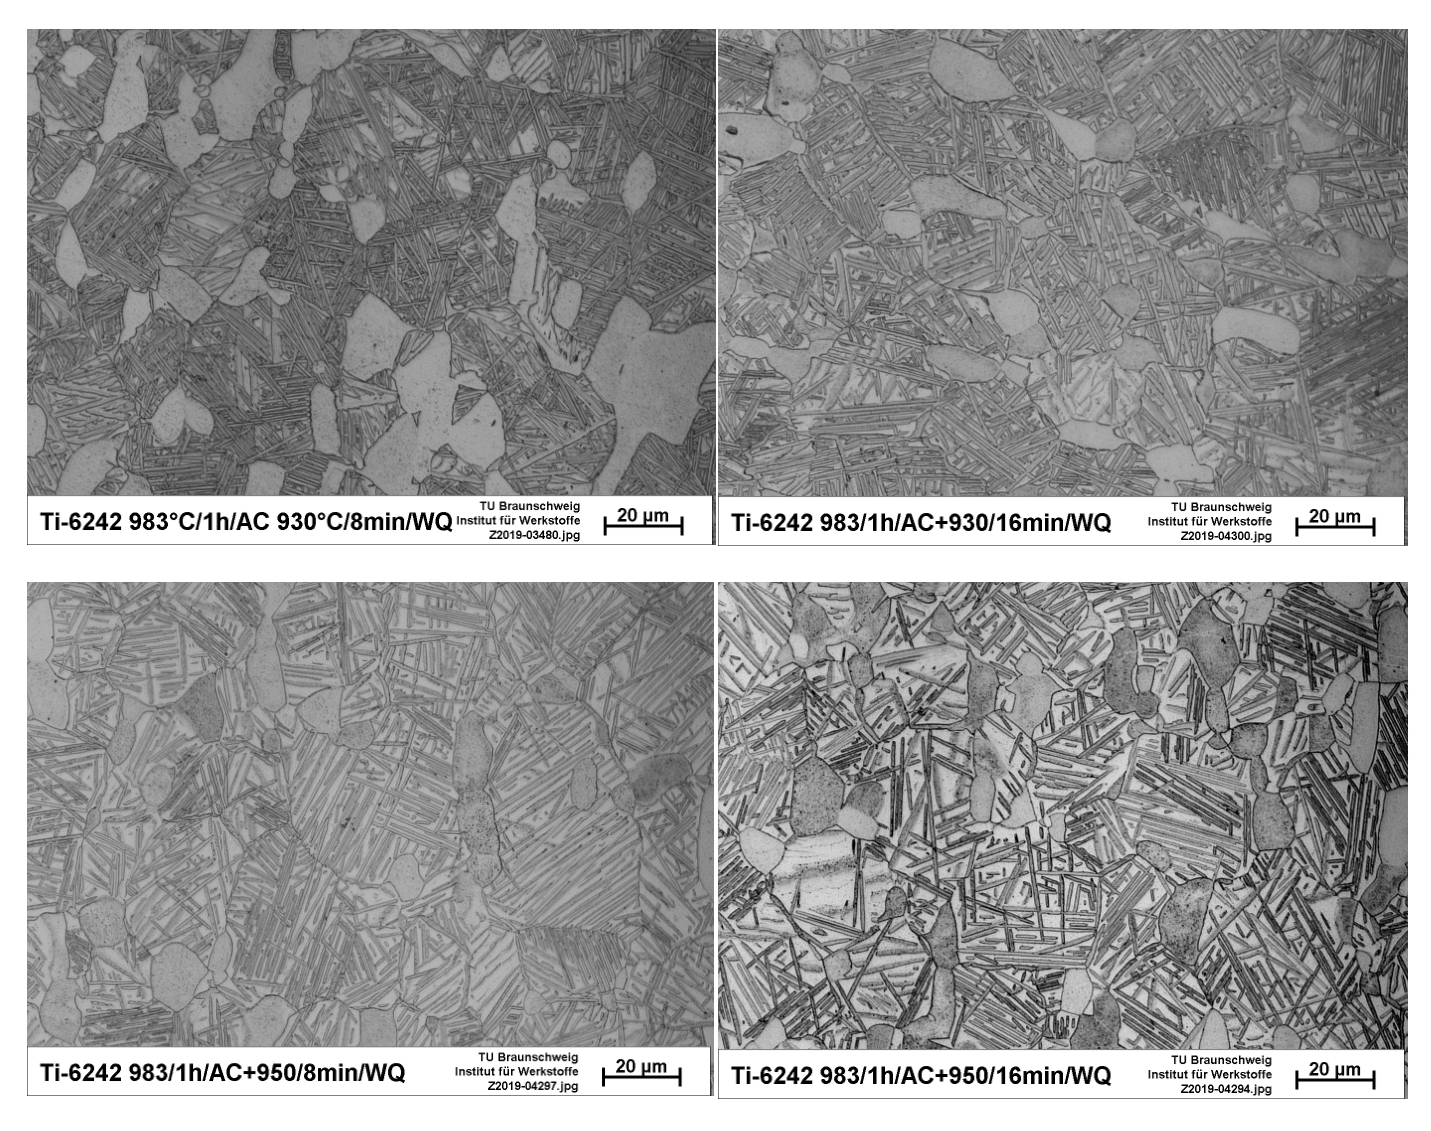
\includegraphics[width=0.9\linewidth]{./Bilder/Abbildung 15}
\caption[Abbildung 15]{Veränderung $\beta$-Phase in zweiten Wärmebehandlungsschritt bei 950$^\circ$C und 930$^\circ$C}
\label{fig:abbildung-15}
\end{figure}

Die Härteprüfung der zweiten Probenreihe mit angepassten Temperaturen und Haltezeiten ergab ebenfalls einen Unterschied zur vorherigen Probenreihe. Die Ergebnisse sind in Tabelle \ref{Tabelle 7} aufgeführt.

\begin{table}
\centering
\begin{tabular}{|c|c|}
\hline 
Probe & Härte in HV \\ 
\hline 
983$^\circ$C/1h/AC + 930$^\circ$C/8min/WQ & 349 \\ 
\hline 
983$^\circ$C/1h/AC + 930$^\circ$C/16min/WQ & 358 \\ 
\hline 
983$^\circ$C/1h/AC + 950$^\circ$C/8min/WQ & 377 \\ 
\hline 
983$^\circ$C/1h/AC + 950$^\circ$C/16min/WQ & 376 \\ 
\hline 
\end{tabular} 
\caption{Ergebnisse der Härteprüfung mit angepassten Temperaturen und Haltezeiten}
\label{Tabelle 7}
\end{table}

Die Härtewerte der Proben, die bei 950$^\circ$C geglüht wurden, weisen eine sichtbare Härtesteigerung gegenüber den Proben, die bei 930$^\circ$C geglüht wurden, auf. Der Wert der Probe, die bei 930$^\circ$C und 16 min geglüht wurde, gegenüber der Probe mit gleicher Temperatur und halber Haltezeit, ist im Rahmen der Genauigkeit nahezu gleich. So zeigt sich, dass in dieser Probenreihe die Haltezeit keinen sichtbaren Einfluss hat. Die nähere Analyse der Mikrostruktur dieser Probenreihe unter dem REM ist in den Abbildungen \ref{fig:abbildung-16} -- \ref{fig:abbildung-18} aufgeführt.

\begin{figure}
	\centering
	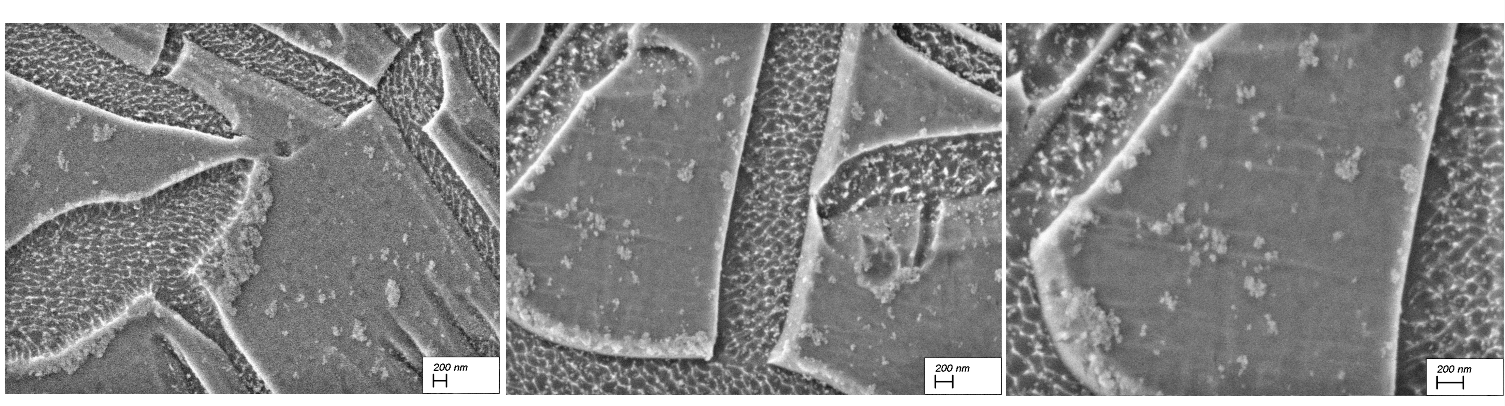
\includegraphics[width=1.0\linewidth]{./Bilder/Abbildung 16}
	\caption[Abbildung 16]{983$^\circ$C/1h/AC + 930$^\circ$C/16min/WQ, REM}
	\label{fig:abbildung-16}
\end{figure}

\begin{figure}
	\centering
	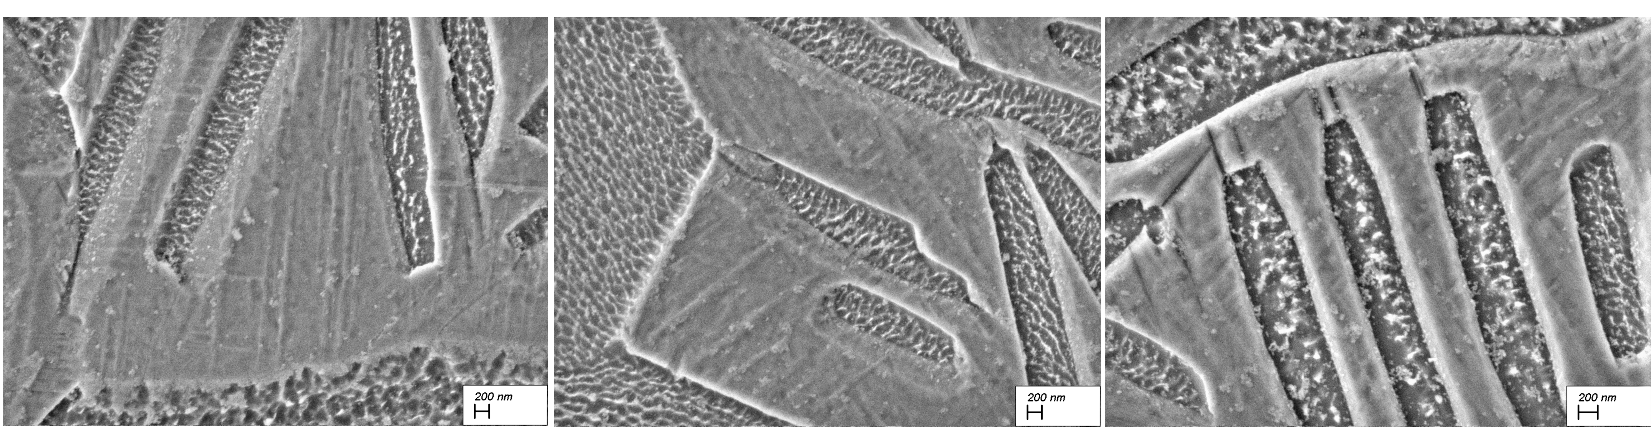
\includegraphics[width=1.0\linewidth]{./Bilder/Abbildung 17}
	\caption[Abbildung 17]{983$^\circ$C/1h/AC + 950$^\circ$C/8min/WQ, REM}
	\label{fig:abbildung-17}
\end{figure}

\begin{figure}
	\centering
	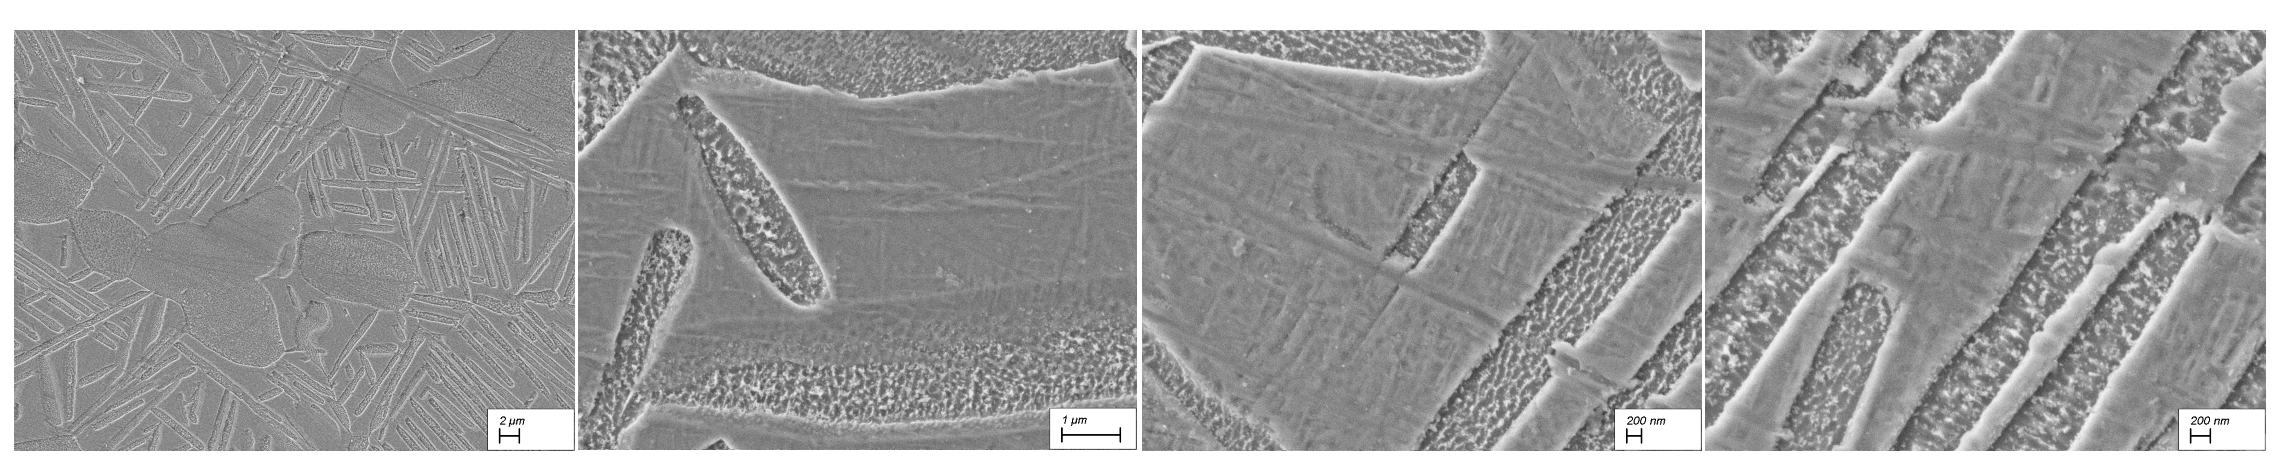
\includegraphics[width=1.0\linewidth]{./Bilder/Abbildung 18}
	\caption[Abbildung 18]{983$^\circ$C/1h/AC + 950$^\circ$C/16min/WQ, REM}
	\label{fig:abbildung-18}
\end{figure}

Die Analyse hat gezeigt, dass auch bei der Probe, die bei 930$^\circ$C für 16 Minuten geglüht wurde, ebenfalls nur im Randbereich an vereinzelten Stellen in der $\beta$-Phase leichte martensitische Strukturen erkennbar waren.
Bei den Proben, die bei einer Temperatur von 950$^\circ$C geglüht wurden, sind über der ganzen Probenfläche ausgeprägte martensitische Strukturen zu erkennen. In den Proben mit tieferer Temperatur haben sich lediglich vereinzelt martensitische Strukturen in Bereichen großflächiger $\beta$-Phase im Randbereich gebildet. Bei den Proben, die bei höherer Temperatur geglüht wurden, haben sich auch in den dünneren Flächen der $\beta$-Phase, die zwischen den $\alpha$-Lamellen liegen, ausgeprägte Martensitstrukturen gebildet.

Im dem dritten Schritt war der Zerfall des Martensits, dass vorher gebildet wurde, geplant. Dazu wurde die Probe aus Abbildung \ref{fig:abbildung-18} (983$^\circ$C/1h/AC + 950$^\circ$C/16min/WQ), die die ausgeprägtesten Martensitstrukturen aufwies, für die weiteren Schritte ausgewählt. 
Dafür wurden vier Proben für den dritten Wärmebehandlungsschritt festgelegt. Zwei Proben wurden bei 580$^\circ$C und unterschiedlichen Haltezeiten (8 und 16 min) wärmebehandelt. Die zwei verbliebenen wurden den gleichen Haltezeiten ausgesetzt, nur bei höher Temperatur (610$^\circ$C).

Die Analyse unter dem Lichtmikroskop ergab keine sichtbare Veränderung der Mikrostruktur zur dritten Probenreihe. Die Ergebnisse der weiteren Auswertung unter dem REM sind in den Abbildungen \ref{fig:abbildung-22} -- \ref{fig:abbildung-25} zusammengefasst.

\begin{figure}
	\centering
	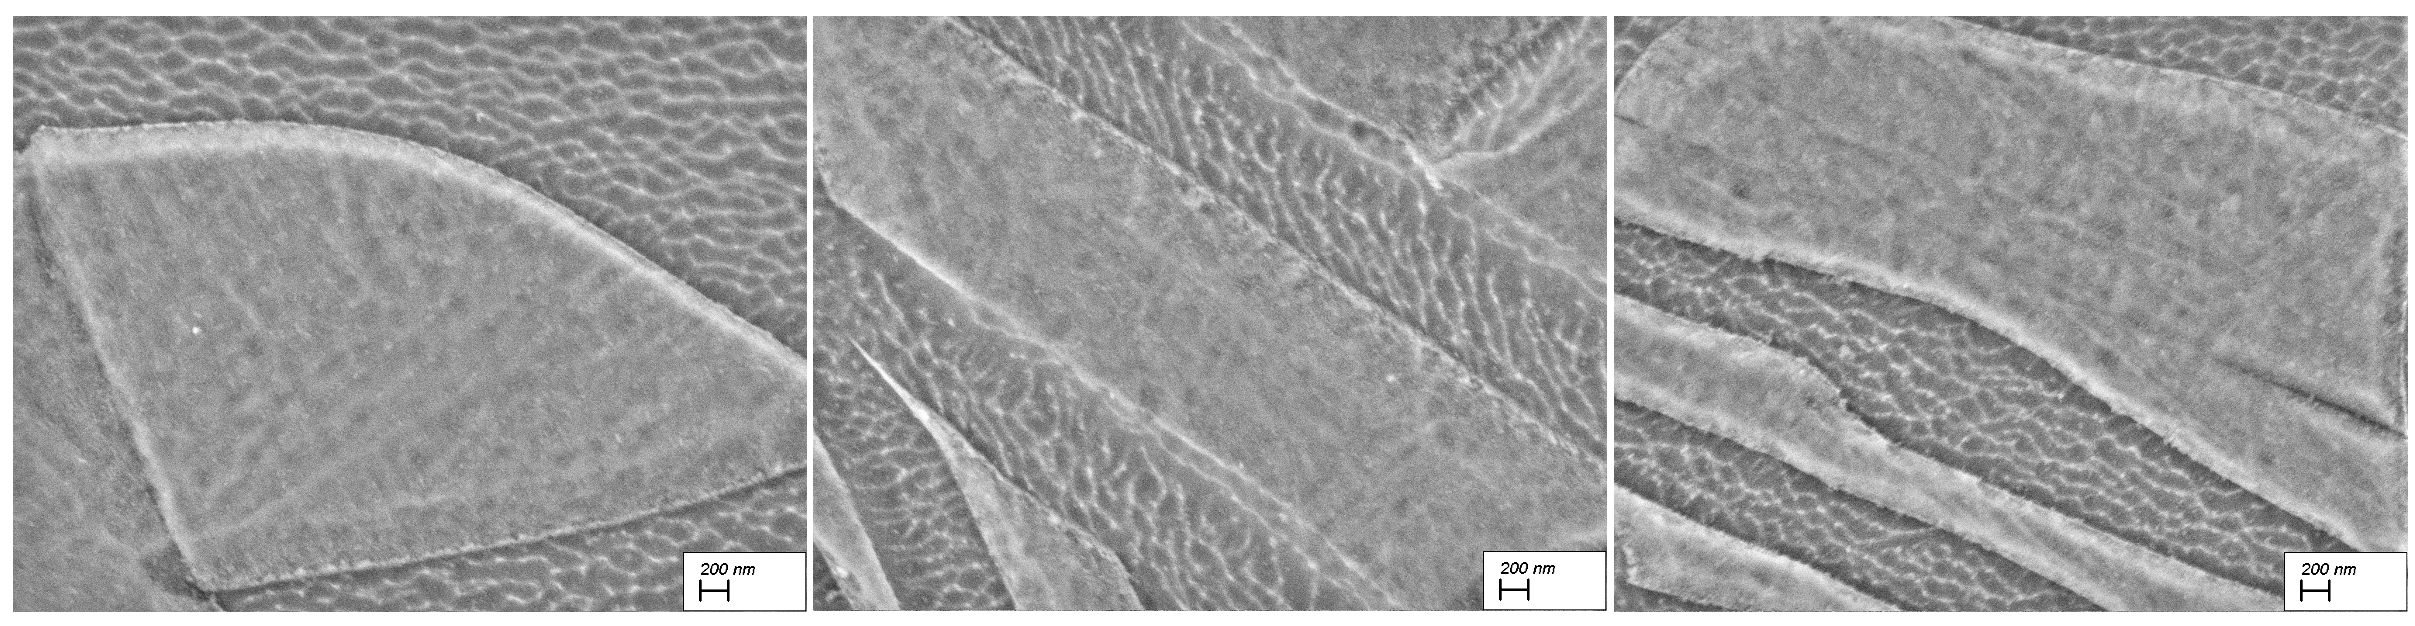
\includegraphics[width=1.0\linewidth]{./Bilder/Abbildung 22.png}
	\caption[Abbildung 22]{983$^\circ$C/1h/AC + 950$^\circ$C/16min/WQ + 580$^\circ$C/8min/AC, REM}
	\label{fig:abbildung-22}
\end{figure}

\begin{figure}
	\centering
	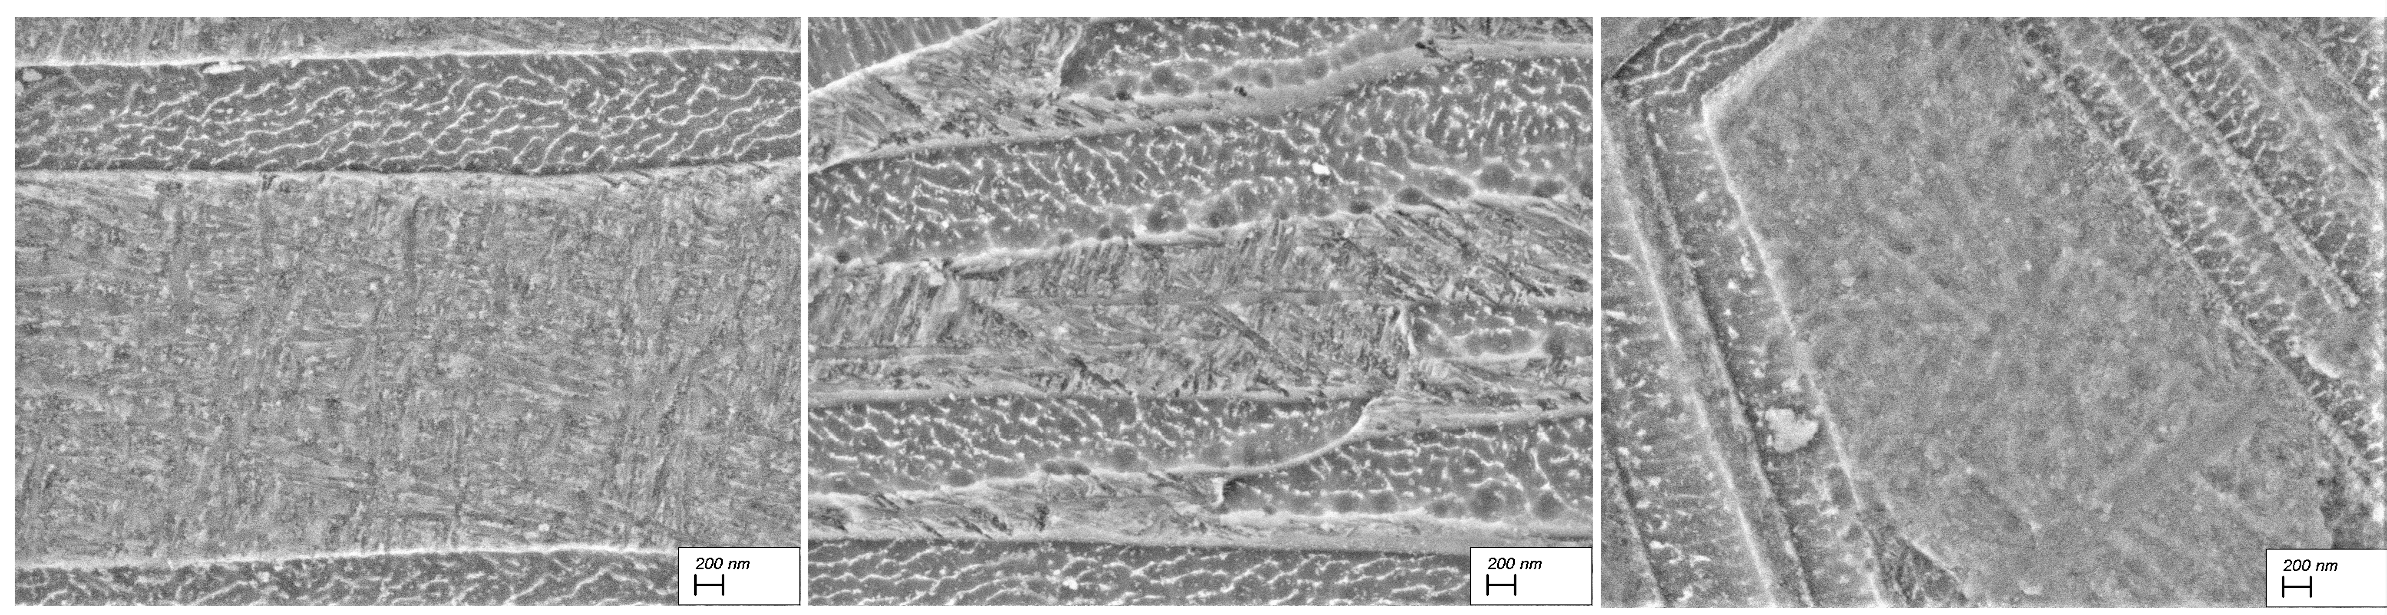
\includegraphics[width=1.0\linewidth]{./Bilder/Abbildung 23.png}
	\caption[Abbildung 23]{983$^\circ$C/1h/AC + 950$^\circ$C/16min/WQ + 580$^\circ$C/16min/AC, REM}
	\label{fig:abbildung-23}
\end{figure}

\begin{figure}
	\centering
	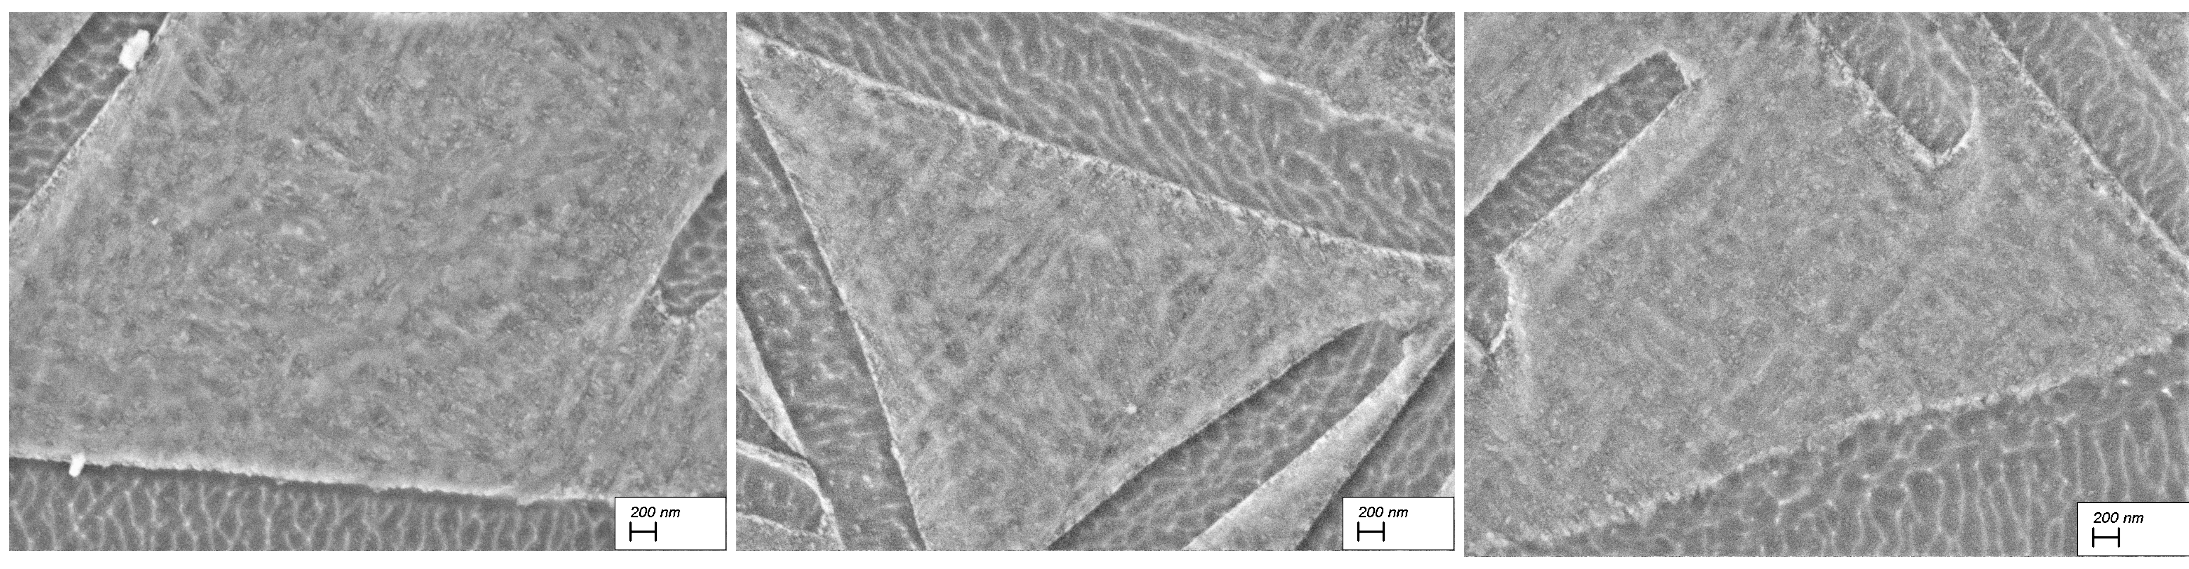
\includegraphics[width=1.0\linewidth]{./Bilder/Abbildung 24.png}
	\caption[Abbildung 24]{983$^\circ$C/1h/AC + 950$^\circ$C/16min/WQ + 610$^\circ$C/8min/AC, REM}
	\label{fig:abbildung-24}
\end{figure}

\begin{figure}
	\centering
	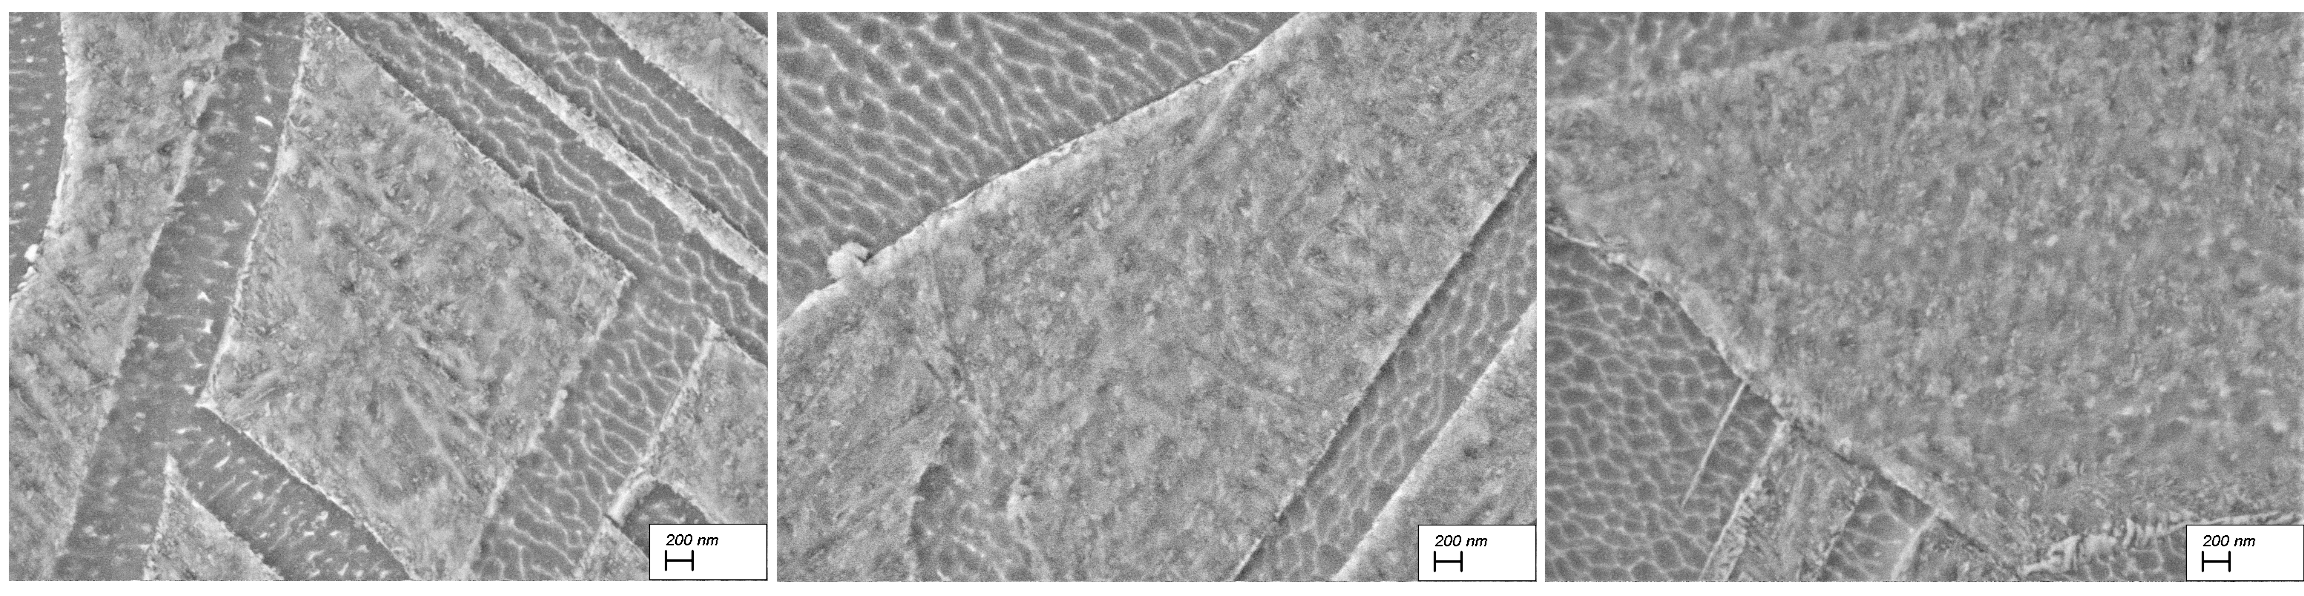
\includegraphics[width=1.0\linewidth]{./Bilder/Abbildung 25.png}
	\caption[Abbildung 25]{983$^\circ$C/1h/AC + 950$^\circ$C/16min/WQ + 610$^\circ$C/16min/AC, REM}
	\label{fig:abbildung-25}
\end{figure}

In den Abbildungen \ref{fig:abbildung-22} -- \ref{fig:abbildung-25} ist zu sehen, dass die Martensitstrukturen in der $\beta$-Phase zum größten Teil zerfallen sind. Nur an vereinzelten Stellen der Proben sind noch ansatzweise Rückstände dieser Strukturen zu erkennen.

Die Härteprüfung zeigte im Gegensatz zur dritten Probenreihe eine sichtbare Härtesteigerung. Die Ergebnisse sind in Tabelle \ref{Tabelle 8} zusammengefasst.

\begin{table}
	\centering
	\begin{tabular}{|c|c|}
		\hline 
		Probe & Härte in HV \\ 
		\hline 
		983$^\circ$C/1h/AC + 950$^\circ$C/16min/WQ + 580$^\circ$C/8min/AC & 393 \\ 
		\hline 
		983$^\circ$C/1h/AC + 950$^\circ$C/16min/WQ + 580$^\circ$C/16min/AC & 392 \\ 
		\hline 
		983$^\circ$C/1h/AC + 950$^\circ$C/16min/WQ + 610$^\circ$C/8min/AC & 399 \\ 
		\hline 
		983$^\circ$C/1h/AC + 950$^\circ$C/16min/WQ + 610$^\circ$C/16min/AC & 392 \\ 
		\hline 
	\end{tabular} 
	\caption{Ergebnisse der Härteprüfung mit angepassten Temperaturen und Haltezeiten}
	\label{Tabelle 8}
\end{table}

\section{$\alpha_p$ - $\alpha'$-Wärmebehandlung (PH)}

Zum Vergleich wurde parallel eine $\alpha_p$ - $\alpha'$ Wärmebehandlung durchgeführt. Im Gegensatz zur der im Abschnitt 5.2. durchgeführten Wärmebehandlung, besitzt diese nur zwei Behandlungsschritte.
Dazu wurde wieder die aus der $\alpha_p$-Studie hervorgegangene Temperatur von 983$^\circ$C ausgewählt, eine Probe für 1 Stunde geglüht und anschließend wassergekühlt. Die dadurch entstandene Mikrostruktur wurde unter dem Lichtmikroskop ausgewertet und ist in Abbildung \ref{fig:abbildung-19} aufgeführt.

\begin{figure}
	\centering
	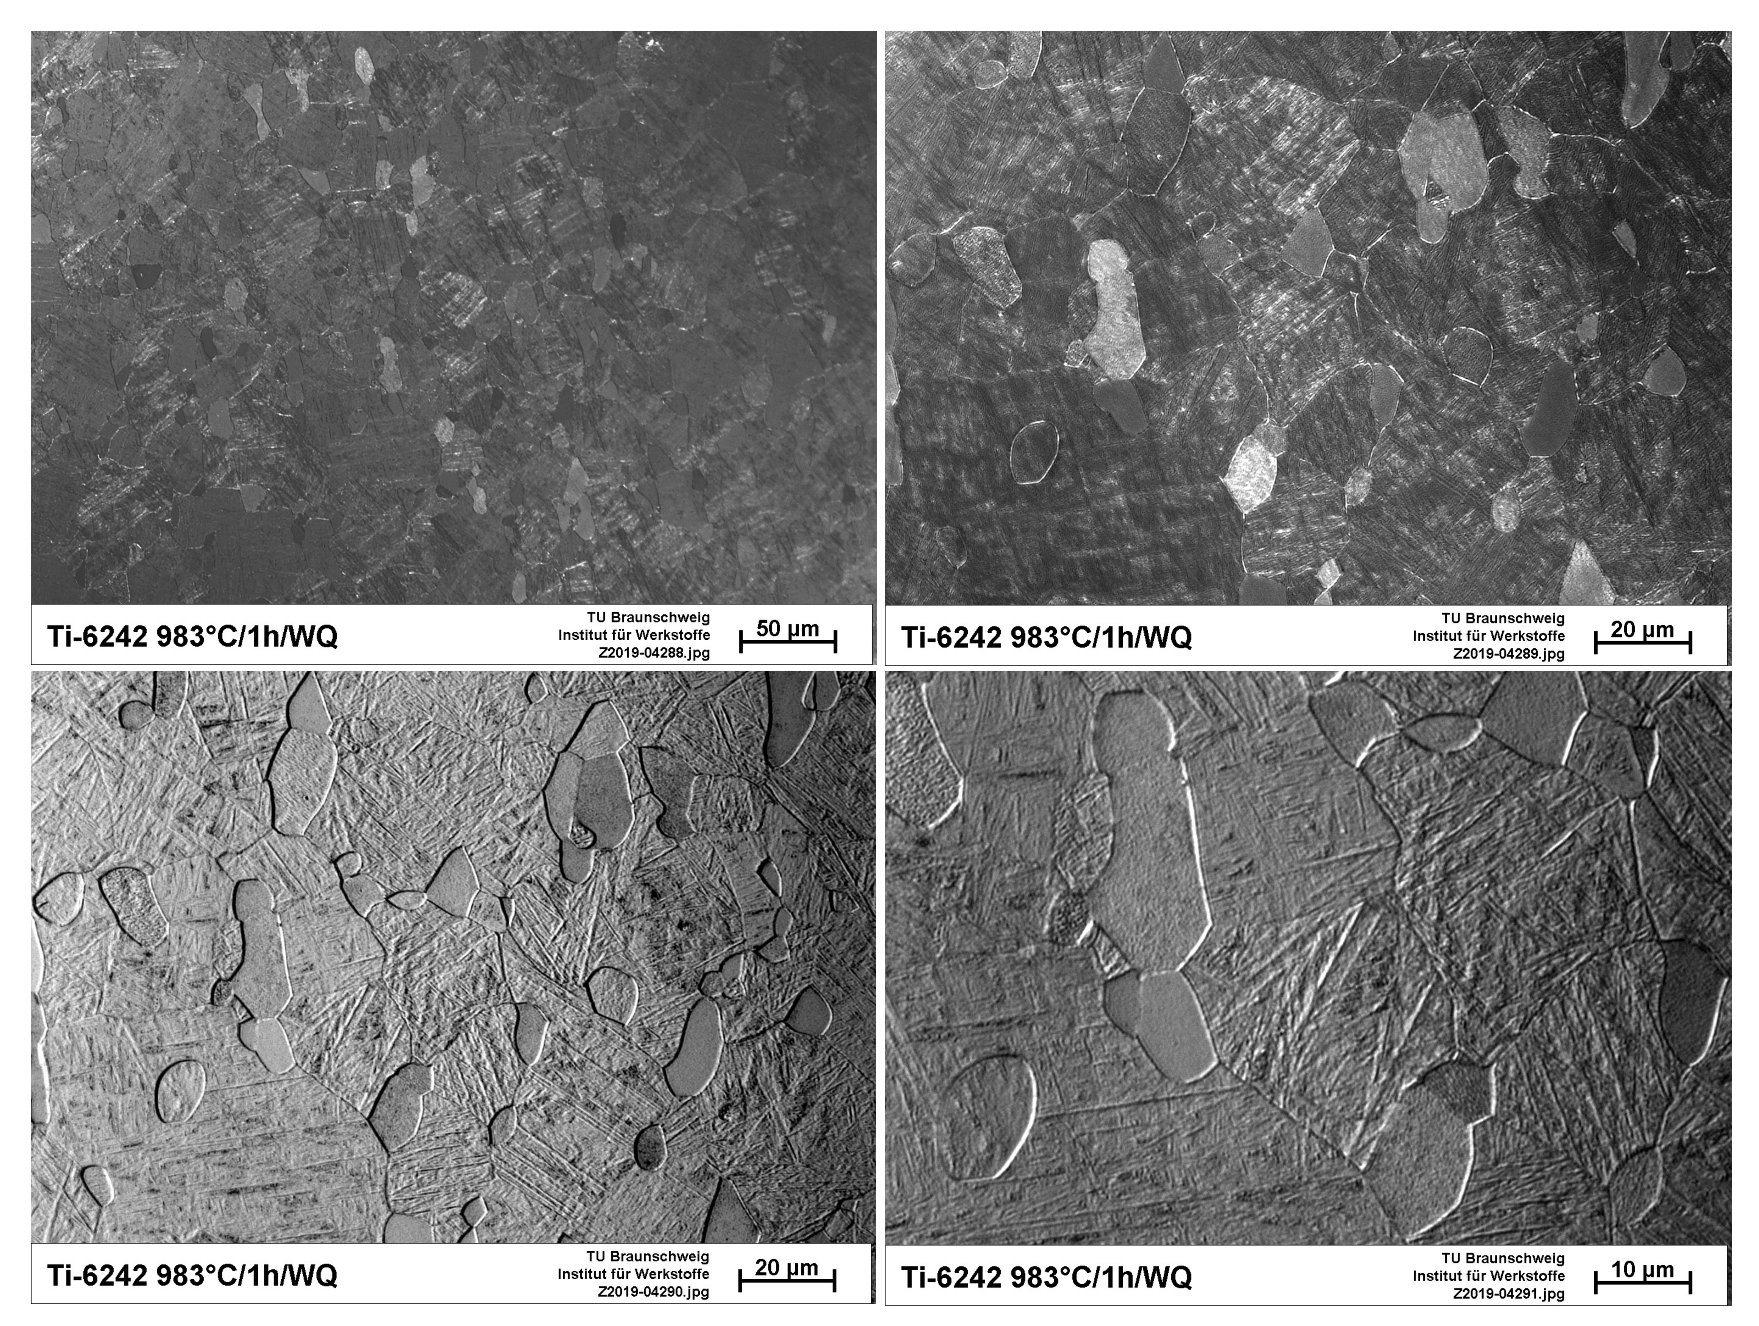
\includegraphics[width=0.9\linewidth]{./Bilder/Abbildung 19}
	\caption[Abbildung 19]{$\alpha_p$ - $\alpha$' Gefüge unter dem Lichtmikroskop bei verschiedenen Vergrößerungen}
	\label{fig:abbildung-19}
\end{figure}

Der Unterschied in diesem ersten Schritt der Wärmebehandlung zu der Behandlung aus Abschnitt 5.2, liegt in der Wasserabkühlung. Das dadurch entstandene Gefüge besteht aus Primär-$\alpha$-Phase ($\alpha_p$) und Martensit ($\alpha'$), das als $\alpha_p$/$\alpha'$-Gefüge bezeichnet wird.

Die anschließende Härteprüfung ergab eine mittlere Vickershärte von 405 HV.

Im zweiten Schritt sollte wieder ein Martensitzerfall durchgeführt werden. Dazu wurden zwei Proben erneut bei 610$^\circ$C wärmebhandelt. Es wurden zwei Haltezeiten 16 und 30 min ausgewählt, mit anschließender Luftabkühlung. Die Auswertung unter dem REM ist in den Abbildungen \ref{fig:abbildung-26} und \ref{fig:abbildung-27} zusammengefasst.

\begin{figure}
	\centering
	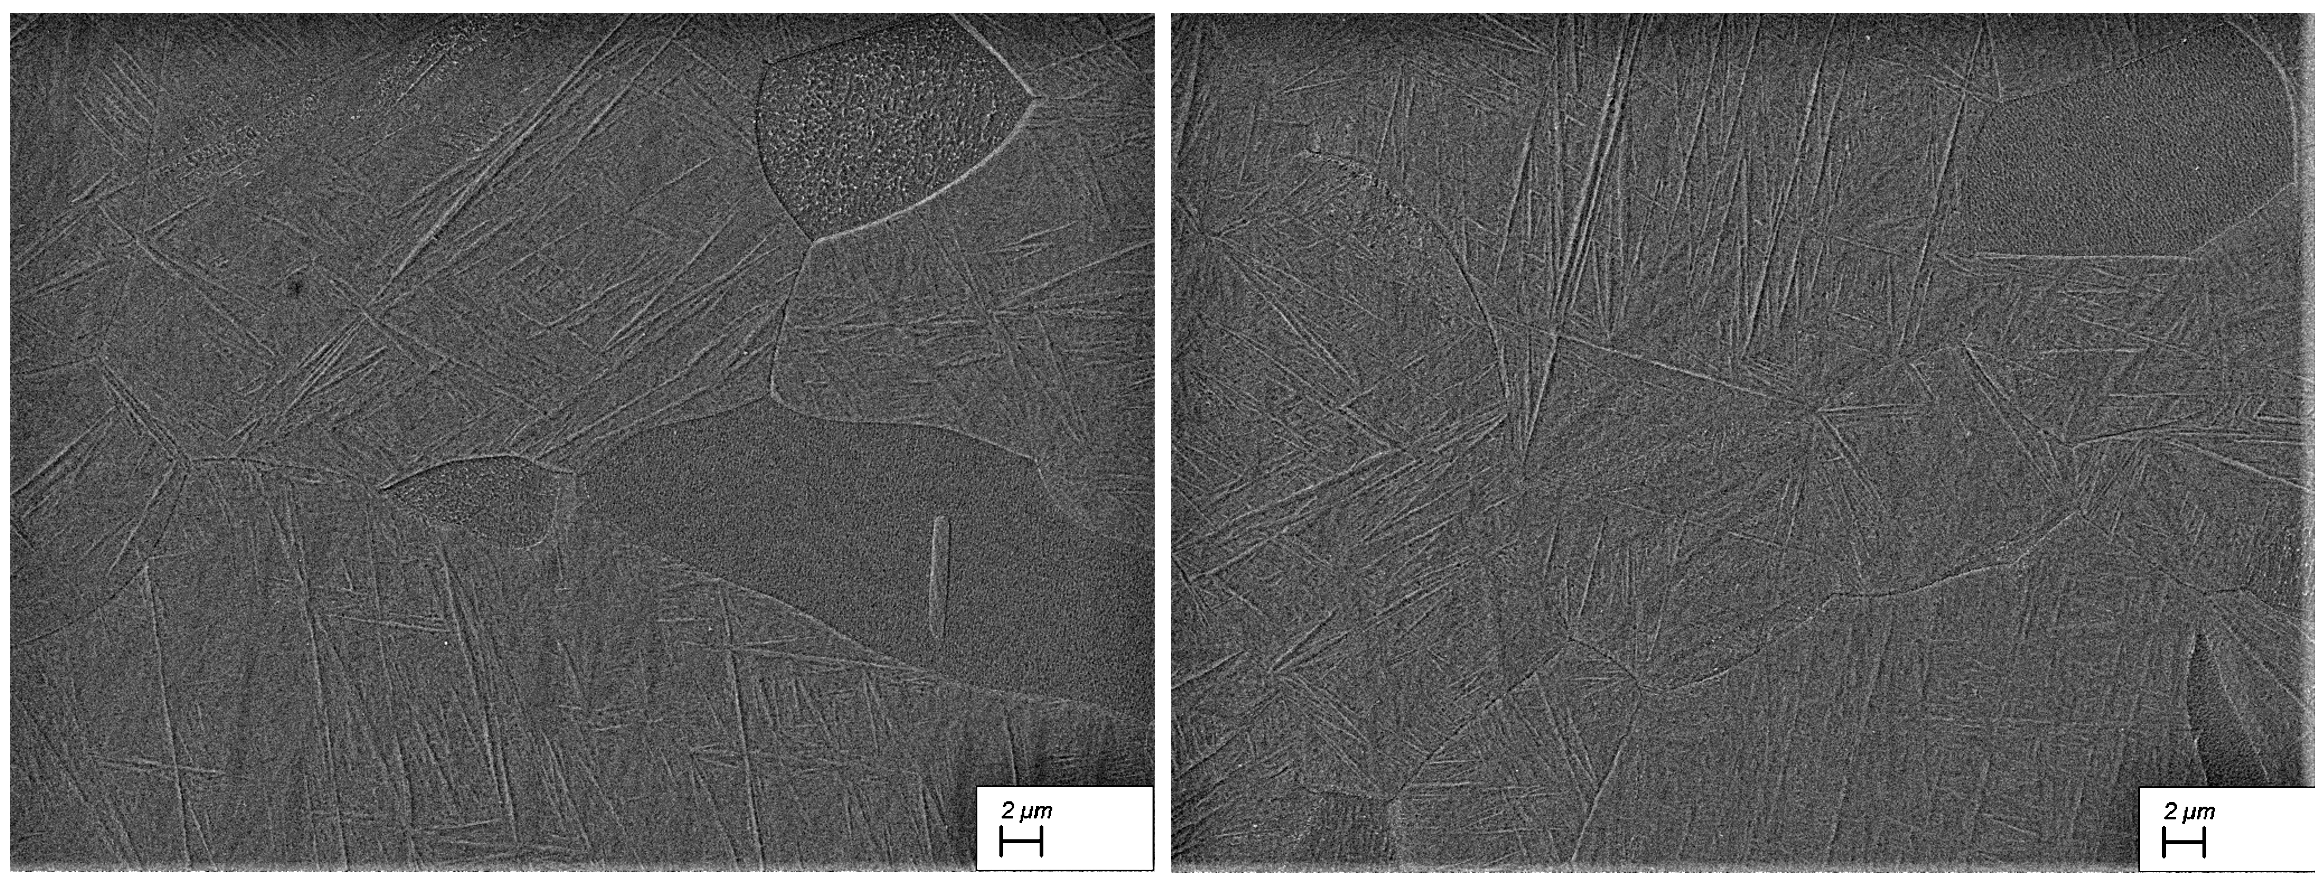
\includegraphics[width=1.0\linewidth]{./Bilder/Abbildung 26.png}
	\caption[Abbildung 26]{983$^\circ$C/1h/WQ + 610$^\circ$C/16min/AC, REM}
	\label{fig:abbildung-26}
\end{figure}

\begin{figure}
	\centering
	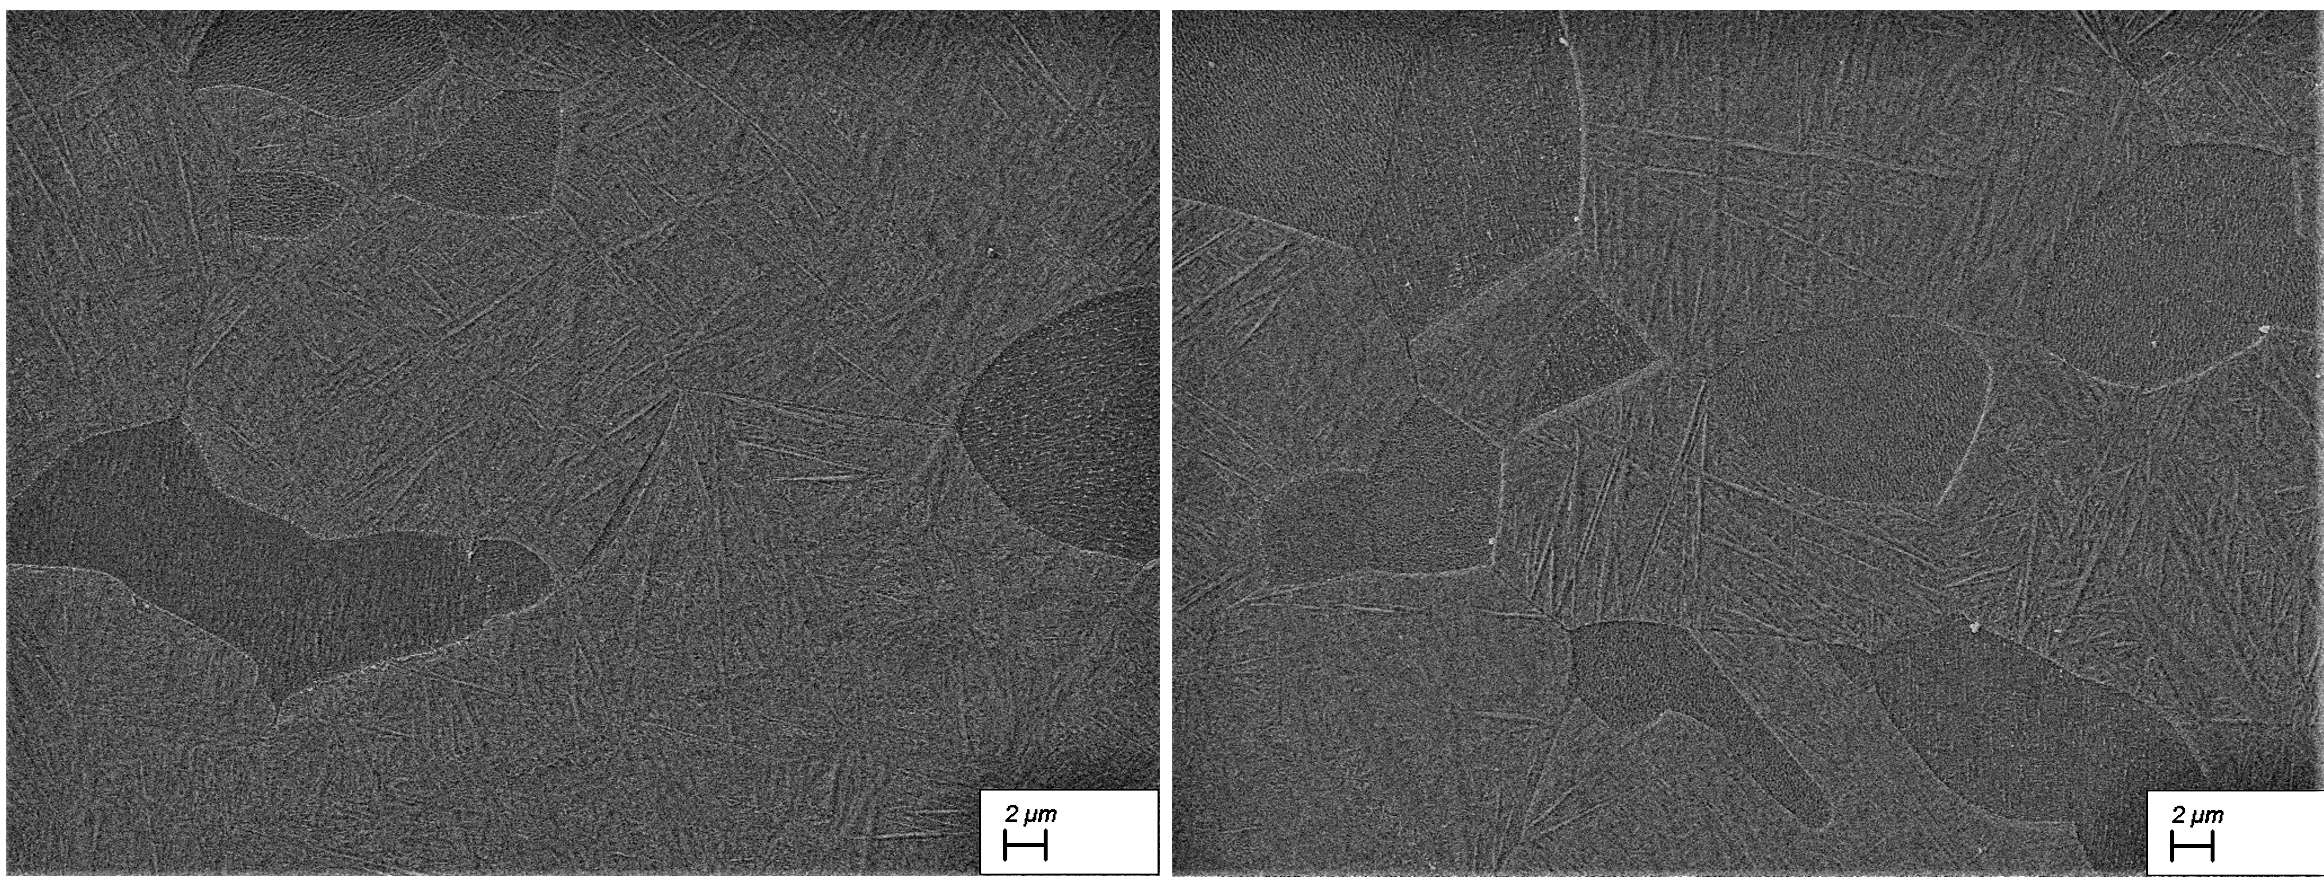
\includegraphics[width=1.0\linewidth]{./Bilder/Abbildung 27.png}
	\caption[Abbildung 27]{983$^\circ$C/1h/WQ + 610$^\circ$C/30min/AC, REM}
	\label{fig:abbildung-27}
\end{figure}

In den Abbildungen \ref{fig:abbildung-26} und \ref{fig:abbildung-27} ist zu erkennen, dass keine Veränderung in dem Gefüge im Vergleich zum vorherigen Schritt feststellbar ist. Es kann davon ausgegangen werden, dass der geplante Martensitzerfall nicht stattgefunden hat.

Die Ergebnisse der Härteprüfung nach diesem zweiten Schritt sind in Tabelle \ref{Tabelle 9} aufgeführt.

\begin{table}
	\centering
	\begin{tabular}{|c|c|}
		\hline 
		Probe & Härte in HV \\ 
		\hline 
		983$^\circ$C/1h/WQ + 610$^\circ$C/16min/AC & 405 \\ 
		\hline 
		983$^\circ$C/1h/WQ + 610$^\circ$C/30min/AC & 400 \\ 
		\hline 
	\end{tabular} 
	\caption{Ergebnisse der Härteprüfung nach der zweiten Wärmebehandlung, $\alpha_p$ - $\alpha'$ Gefüge}
	\label{Tabelle 9}
\end{table}

Es ist zu erkennen, dass auch die Härte unverändert im Vergleich zum vorherigen Schritt blieb.
